% This LaTeX document needs to be compiled with XeLaTeX.
\documentclass[
  10
]{article}
\usepackage[margin=2cm,includehead=true,includefoot=true,centering,]{geometry}
\usepackage{xcolor}
\usepackage{ucharclasses}
\usepackage{hyperref}
\usepackage{amsmath,amssymb}
\usepackage{amsfonts}
\usepackage[version=4]{mhchem}
\usepackage{stmaryrd}
\usepackage{bbold}
\usepackage{polyglossia}
\usepackage{fontspec}
\usepackage{ctex}
\usepackage[export]{adjustbox}
\usepackage{tabularx}
\usepackage{booktabs}

\usepackage{setspace}
\setstretch{1.2}

\makeatletter
\@ifundefined{KOMAClassName}{% if non-KOMA class
  \IfFileExists{parskip.sty}{%
    \usepackage{parskip}
  }{% else
    \setlength{\parindent}{0pt}
    \setlength{\parskip}{6pt plus 2pt minus 1pt}}
}{% if KOMA class
  \KOMAoptions{parskip=half}}
\makeatother
\usepackage{longtable,booktabs,array}
\usepackage{multirow}
\usepackage{calc} % for calculating minipage widths
% Correct order of tables after \paragraph or \subparagraph
\usepackage{etoolbox}
\makeatletter
\patchcmd\longtable{\par}{\if@noskipsec\mbox{}\fi\par}{}{}
\makeatother
% Allow footnotes in longtable head/foot
\IfFileExists{footnotehyper.sty}{\usepackage{footnotehyper}}{\usepackage{footnote}}
\makesavenoteenv{longtable}
\usepackage{graphicx}
\makeatletter
\newsavebox\pandoc@box
\newcommand*\pandocbounded[1]{% scales image to fit in text height/width
  \sbox\pandoc@box{#1}%
  \Gscale@div\@tempa{\textheight}{\dimexpr\ht\pandoc@box+\dp\pandoc@box\relax}%
  \Gscale@div\@tempb{\linewidth}{\wd\pandoc@box}%
  \ifdim\@tempb\p@<\@tempa\p@\let\@tempa\@tempb\fi% select the smaller of both
  \ifdim\@tempa\p@<\p@\scalebox{\@tempa}{\usebox\pandoc@box}%
  \else\usebox{\pandoc@box}%
  \fi%
}
% Set default figure placement to htbp
\def\fps@figure{htbp}
\makeatother
\setlength{\emergencystretch}{3em} % prevent overfull lines
\providecommand{\tightlist}{%
  \setlength{\itemsep}{0pt}\setlength{\parskip}{0pt}}


\hypersetup{colorlinks=true, linkcolor=blue, filecolor=magenta, urlcolor=cyan,}
\urlstyle{same}

\usepackage{colortbl}
\definecolor{table-row-color}{HTML}{999999}
\definecolor{table-rule-color}{HTML}{999999}
%\arrayrulecolor{black!40}
\arrayrulecolor{table-rule-color}     % color of \toprule, \midrule, \bottomrule
\setlength{\aboverulesep}{0pt}
\setlength{\belowrulesep}{0pt}


\setotherlanguages{english}
\IfFontExistsTF{Source Han Serif CN}
{\newfontfamily\chinesefont{Source Han Serif CN}}
{\IfFontExistsTF{Noto Serif CJK SC}
  {\newfontfamily\chinesefont{Noto Serif CJK SC}}
  {\IfFontExistsTF{SimSun}
    {\newfontfamily\chinesefont{SimSun}}
    {\IfFontExistsTF{FangSong}
      {\newfontfamily\chinesefont{FangSong}}
      {\newfontfamily\chinesefont{Arial Unicode MS}}
}}}
\IfFontExistsTF{Times New Roman}
{\newfontfamily\englishfont{Times New Roman}}
{\IfFontExistsTF{Liberation Serif}
  {\newfontfamily\englishfont{Liberation Serif}}
  {\IfFontExistsTF{DejaVu Serif}
    {\newfontfamily\englishfont{DejaVu Serif}}
    {\newfontfamily\englishfont{Arial}}
}}


\author{}
\date{}

\begin{document}


\section{《模拟电子技术基础实验》}\label{ux6a21ux62dfux7535ux5b50ux6280ux672fux57faux7840ux5b9eux9a8c}

\section{实验报告}\label{ux5b9eux9a8cux62a5ux544a}

\pandocbounded{
\includegraphics[keepaspectratio]{images/ab3a6e2371da0370ea4875dcfcbc9693b9a34829f7dace9ce83bbb91cb1091f8.jpg}}

学 院： 微电子学院

学号: 2023303118 2023303120

姓名： 徐洋坤 王澜溪

实验组号： 38

2025年1月

\section{目录}\label{ux76eeux5f55}

实验一、二 单极共射放大器 4

一、实验目的 4\\
二、实验原理 4\\
三、实验内容 6\\
四、实验电路方案 6\\
五、测试与数据记录 6\\
六、结论与分析 10

实验三、运算放大器类型与主要指标 11

一、实验目的 11\\
二、实验原理 11\\
三、实验内容 11\\
四、实验电路方案 12\\
五、测试与数据记录 12\\
六、结论与分析 14

实验四、运算放大器线性应用 15

一、实验目的 15\\
二、实验原理 15\\
三、实验内容 15\\
四、实验电路方案 15\\
五、测试与数据记录 16\\
六、结论与分析 18

实验五、正弦波振荡电路 19

一、实验目的 19\\
二、实验原理 19\\
三、实验内容 19\\
四、实验电路方案 19\\
五、测试与数据记录 20\\
六、结论与分析 24

实验六、有源滤波器 24

一、实验目的 24\\
二、实验原理 25\\
三、实验内容 25\\
四、实验电路方案 26\\
五、测试与数据记录 27\\
六、结论与分析 28

实验七、全波整流滤波 28

一、实验目的 28\\
二、实验原理 28\\
三、实验内容 29\\
四、实验电路方案 29\\
五、测试与数据记录 29\\
六、结论与分析 30

实验八、功率放大电路 31

一、实验目的 31\\
二、实验原理 31\\
三、实验内容 31\\
四、实验电路方案 32\\
五、测试与数据记录 32\\
六、结论与分析 33

\pandocbounded{
\includegraphics[keepaspectratio]{images/511e502146d08bf7e3aa1ef53ee7b0352ea670fc80b0f6cee6efc629e7543837.jpg}}

\section{实验一、二
单极共射放大器}\label{ux5b9eux9a8cux4e00ux4e8c-ux5355ux6781ux5171ux5c04ux653eux5927ux5668}

\section{一、实验目的}\label{ux4e00ux5b9eux9a8cux76eeux7684}

1、分析静态工作点对放大器性能的影响，学会调试放大器的静态工作点。\\
2、掌握放大器电压放大倍数、输入电阻、输出电阻及最大不失真输出电压的测量方法。\\
3、掌握放大电路的频率特性。

\section{二、实验原理}\label{ux4e8cux5b9eux9a8cux539fux7406}

\section{1、基本共射放大电路}\label{ux57faux672cux5171ux5c04ux653eux5927ux7535ux8def}

输入信号加在三极管的基极,输出信号由集电极取出,发射极作为输入回路和输出回路的公共电极时的放大电路,称为基本共射极放大电路。放大作用是利用BJT的基极对集电极的控制作用来实现的,即在输入端加一个能量较小的信号,通过BJT的基极电流控制流过集电极电路的电流,从而将直流电源
\(V_{CC}\)
的能量转化为所需要的形式供给负载。为稳定放大器的静态工作点,采用基极固定分压式偏置电路,本实验原理图如图1所示。

\pandocbounded{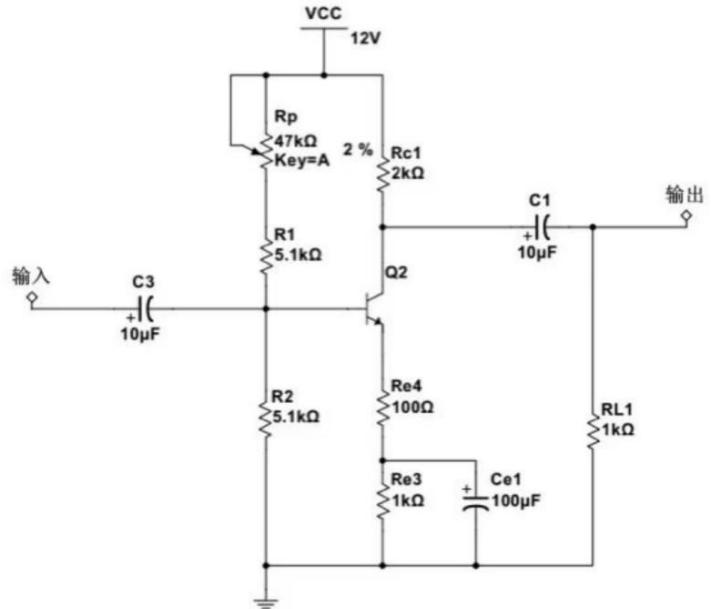
\includegraphics[keepaspectratio]{images/cd4d961e5c5a0d5b5b812810162c0d703845f56364ebd39cb767c631a8b83fc4.jpg}}\\
图1单级共射放大电路

\section{2、静态工作点的选择}\label{ux9759ux6001ux5de5ux4f5cux70b9ux7684ux9009ux62e9}

放大器静态工作点的选择是指对三极管集电极电流 \(I_{C}\)
的调整与测试。在晶体管低频放大电路中，静态工作点的选择及稳定具有举足轻重的作用,直接关系到放大电路能否正常可靠地工作，对于NPN型三极管：

若工作点偏高 \((I_{C}\)
放大)，则放大器在加入交流信号以后易产生饱和失真，此时输出信号 \(u_{o}\)
的负半周将被削底；若工作点偏低，则易产生截止失真，即 \(u_{o}\)
的正半周被削顶，这些情况都不符合不失真放大的要求。

所以在选定静态工作点以后还必须进行动态调试,即在放大器的输入端加入一定的输入电压，并检查输出电压的大小和波形是否满足要求。如不满足，则应调节静态工作点的位置。

此外，如果信号幅度很小，则即使工作点较高或较低也不一定会出现失真。所以确切地说产生波形失真是信号幅度与静态工作点设置配合不当所致。若须满足较大信号幅度的要求，则静态工作点最好尽量靠近输出特性曲线上交流负载线的中点，如图2所示的Q点，使静态
\(\mathbf{u}_{\mathrm{CE}}\)
大致等于电源电压的一半。这样可使交流信号输人时，工作点Q沿着交流负载线向上或向下移动较大范围，使得输出电压的动态范围大致在
\(2u_{CEQ}\) 范围内变化，从而获得较大的输出电压幅度，且波形上下对称。

\pandocbounded{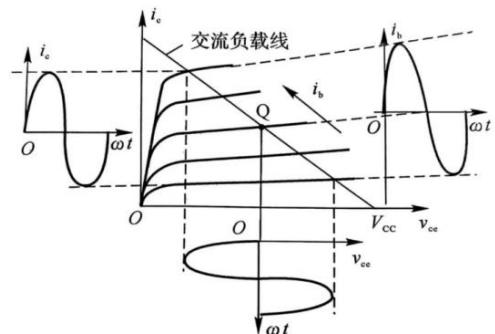
\includegraphics[keepaspectratio]{images/0809f6e26ea84925e20cb3b83329cdaf54683276ee6f1d0fc83fbb9dcf8cd905.jpg}}\\
图2具有最大动态范围的静态工作点图

\section{3、电压放大倍数的测量}\label{ux7535ux538bux653eux5927ux500dux6570ux7684ux6d4bux91cf}

电压放大倍数是指放大器输出电压 \(V_{o}\) 与输入电压 \(V_{i}\)
之比，其值与负载 \(R_{L}\) 有关，是衡量放大电路放大能力的指标。

\[
A _ {V} = \frac {V _ {o}}{V _ {i}}
\]

\section{4、输入电阻和输出电阻的测量}\label{ux8f93ux5165ux7535ux963bux548cux8f93ux51faux7535ux963bux7684ux6d4bux91cf}

\begin{enumerate}
\def\labelenumi{\arabic{enumi}.}
\tightlist
\item
  输入电阻: 输入电阻是指从放大器输入端看进去的等效电阻,
  它表明放大器对信号源的影响程度, 一般采用间接法进行测量。
\end{enumerate}

当被测电路的输入电阻不太高时(与毫伏级电压表的内阻相比),采用如图3所示的电路进行测量。在信号源与被测放大器的输入端之间串入一已知电阻
\(R\) , 在放大器正常工作的情况下(保证输出电压不失真), 测出 \(V_{s}\) 和
\(V_{i}\) , 根据输入电阻的定义可得

\[
R _ {i} = \frac {V _ {i}}{I _ {i}} = \frac {V _ {i}}{\frac {V _ {R}}{R}} = \frac {V _ {i}}{V _ {s} - V _ {i}} R
\]

测量时应注意,电阻 \(R\) 值不宜取得过大, 易引入干扰; 但也不宜取得过小,
否则测量误差较大。通常取与 \(R_{i}\) 为同一数量级比较合适, 本实验取
\(R = 1 \sim 2 k \Omega\) 。

\pandocbounded{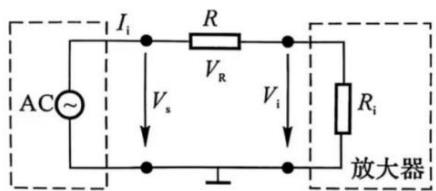
\includegraphics[keepaspectratio]{images/1c0b8c7ca0e6497670000659b994892941586570c3201a86ec6339bb14250a5e.jpg}}\\
图3输入电阻测量原理

\begin{enumerate}
\def\labelenumi{\arabic{enumi}.}
\setcounter{enumi}{1}
\tightlist
\item
  输出电阻: 输出电阻也用间接法测量, 原理如图 4 所示, 根据戴维南定理,
  放大器的输出端可以等效为一个理想的电压源和输出电阻 \(R_{o}\) 相串联。
\end{enumerate}

\pandocbounded{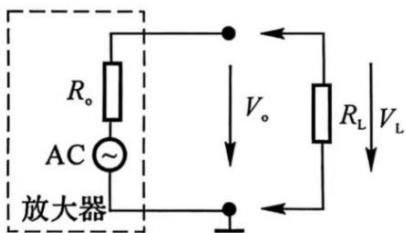
\includegraphics[keepaspectratio]{images/63939b58c9eda331e46ffdb7a491d52ea4a1933622cf10d5800ad01bedc78578.jpg}}\\
图4输出电阻测量原理

实验中可以通过测量放大器空载时的输出电压 \(V_{o}\)
和带已知负载后的输出电压 \(V_{L}\)

由 \(V_{L} = \frac{R_{L}}{R_{o} + R_{L}} V_{o}\) 一式，可得输出电阻
\(R_{o} = \left(\frac{V_{o}}{V_{L}} -1\right)R_{L}\)

\section{5、幅频特性的测量}\label{ux5e45ux9891ux7279ux6027ux7684ux6d4bux91cf}

放大器放大的实际信号由许多频率不同的谐波组成,只有当放大器对不同频率信号的放

大能力相同时,放大信号才能不产生失真。但实际上,放大器的交流放大电路含有耦合电容旁路电容、分布电容和晶体管极间电容等电抗元件,使得放大倍数与信号的频率有关,此关系即为放大器的频率特性。

放大器的幅频特性是指放大器的电压放大倍数 \(A_{V}\) 与输入信号频率
\(f_{i}\)
之间的关系曲线。如图5所示。在一个较宽的频率范围内，曲线平坦，放大倍数不随频率而变，这一段频率范围称为中频段。在中频段以外，随着频率的减小或增大，放大倍数都将下降。当放大倍数下降为中频段放大倍数的0.707时，相对应的低频频率和高频频率分别称为下限额率
\(f_{L}\) 和上限频率 \(f_{H}\) 。通频带 \(f_{BW}\) 定义为

\pandocbounded{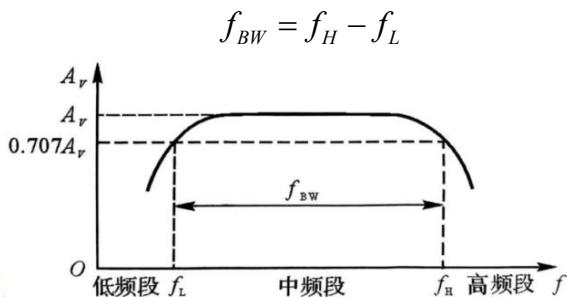
\includegraphics[keepaspectratio]{images/50caecdf81e68c4f38e6541c93cbdae90c95b69401c5c84da9e68549a177c952.jpg}}\\
图5放大器的幅频特性

\section{三、实验内容}\label{ux4e09ux5b9eux9a8cux5185ux5bb9}

1、寻找共射放大电路的静态工作点，即输入信号幅度由小变大时，输出信号由不失真恰好变为同时发生两种失真的状态。\\
2、电压放大倍数测量，使用 \(1 \mathrm{kHz}\)
正弦波作为输入信号，调整输入正弦波幅值和电阻 \(\mathrm{Rp}\)
，找到最佳直流工作点，此时在有载和无载情况下分别计算电压放大倍数
\(A_{V}\) 。\\
3、测量输入电阻和输出电阻。\\
4、测量频幅特性，计算通频带。

\section{四、实验电路方案}\label{ux56dbux5b9eux9a8cux7535ux8defux65b9ux6848}

\pandocbounded{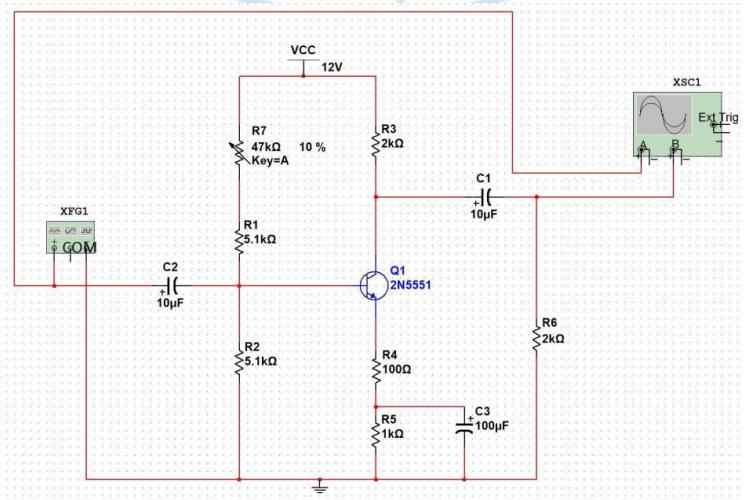
\includegraphics[keepaspectratio]{images/3d4484f4d779fdc7b04a1ff59f38a8def58e9adf08eb78365348ef2c44444b01.jpg}}\\
理论仿真电路（接入负载 \(R_{L} = 2k\Omega\) ）

\section{五、测试与数据记录}\label{ux4e94ux6d4bux8bd5ux4e0eux6570ux636eux8bb0ux5f55}

\section{1. 测试用仪器}\label{ux6d4bux8bd5ux7528ux4eeaux5668}

2N5551型NPN三极管;电阻、电解电容若干;直流电源;示波器;导线若干

\section{2. 实验步骤}\label{ux5b9eux9a8cux6b65ux9aa4}

\section{（1）静态工作点的选择}\label{ux9759ux6001ux5de5ux4f5cux70b9ux7684ux9009ux62e9-1}

使用 \(1 \mathrm{kHz}\) 正弦波作为输入信号, 调整输入正弦波幅值和电阻
\(R_{p}\) , 分别观察截止失真和

饱和失真的波形，并调节 \(R_{p}\)
找到最佳直流工作点（截止失真和饱和失真程度相同，并且减小信号幅度输出完整波形。）

\section{（2）放大倍数的测量}\label{ux653eux5927ux500dux6570ux7684ux6d4bux91cf}

本实验将分别测量有负载与无负载情况的电压放大倍数 \(A_{V}\)

调整到合适的静态工作点后, 输入信号为 \(1 \mathrm{kHz}\) 、幅度为
\(100 \mathrm{mV}\) 的正弦波信号, 接入负载 \(R_{L} = 2 k \Omega\)
方便测量输出电压, 用示波器观察 \(V_{o}\) 和 \(V_{i}\) 的波形,
分别测出电压 \(V_{i}\) 和 \(V_{o}\) 。

\[
\text {代 入 公 式 即 可 计 算} A _ {V} = \frac {V _ {o}}{V _ {i}}
\]

\begin{itemize}
\item
  无负载情况下：开关 \(J_{2}\) 打开
\item
  有负载情况下：开关 \(J_{2}\) 闭合
\end{itemize}

\pandocbounded{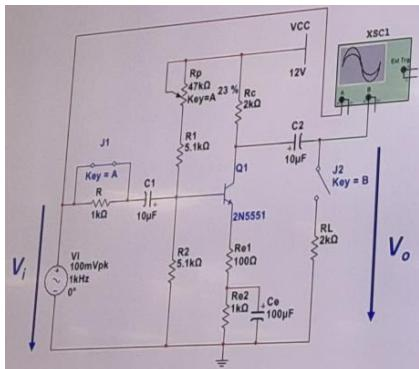
\includegraphics[keepaspectratio]{images/ff1b884eaffbf3791fc027a46fa48a904ad4c8e599e9b1b1789030a5c2e84375.jpg}}

\pandocbounded{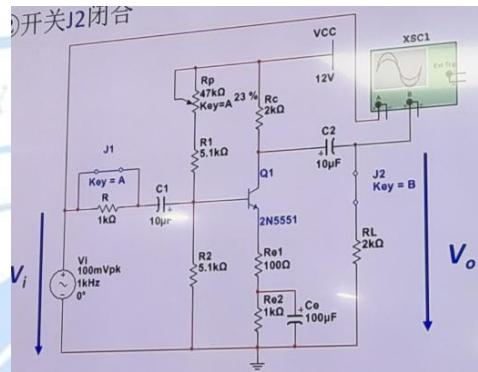
\includegraphics[keepaspectratio]{images/2e6e04be8307dab613f95d486bcb7c5eab31b3848e3eb99e7f34c748bf375030.jpg}}

\section{（3）输入输出电阻测量}\label{ux8f93ux5165ux8f93ux51faux7535ux963bux6d4bux91cf}

·输入电阻

在输入端, 接入电阻 \(R = 1 k \Omega\) , 测量电阻 R 两端的对地电位
\(V_{s}\) 和 \(V_{i}\) , 代入公式即得

\[
R _ {i} = \frac {V _ {i}}{V _ {s} - V _ {i}} R
\]

·输出电阻

测量放大器空载时的输出电压 \(V_{o}\) 与带负载 \(R_{L} = 2 k \Omega\)
后的输出电压 \(V_{L}\) , 代入公式即得

\[
R _ {o} = \left(\frac {V _ {o}}{V _ {L}} - 1\right) R _ {L}
\]

\section{（4）频率特性测量}\label{ux9891ux7387ux7279ux6027ux6d4bux91cf}

保持输入信号幅度不变，改变频率，先测量中频段（选取 \(1\mathrm{kHz}\)
）时的输出电压；在分别降低、提高频率多次试验，当输出电压下降为中频段的0.707倍时，相对应的低频频率和高频频率即为下限额率
\(f_{L}\) 和上限频率 \(f_{H}\) ，并由此计算通频带
\(f_{BW} = f_{H} - f_{L}\) 。

\section{3.
实验结果与数据记录}\label{ux5b9eux9a8cux7ed3ux679cux4e0eux6570ux636eux8bb0ux5f55}

（1）静态工作点波形图（临界不失真与恰好同时发生两种失真）：

\pandocbounded{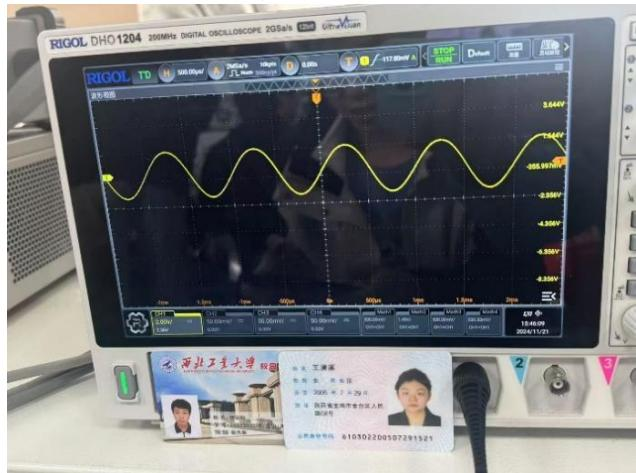
\includegraphics[keepaspectratio]{images/94c0213ebc1d7fc8ca5a1f0c09519de24289f63239e2a85a7460faf9fddc7c16.jpg}}

\pandocbounded{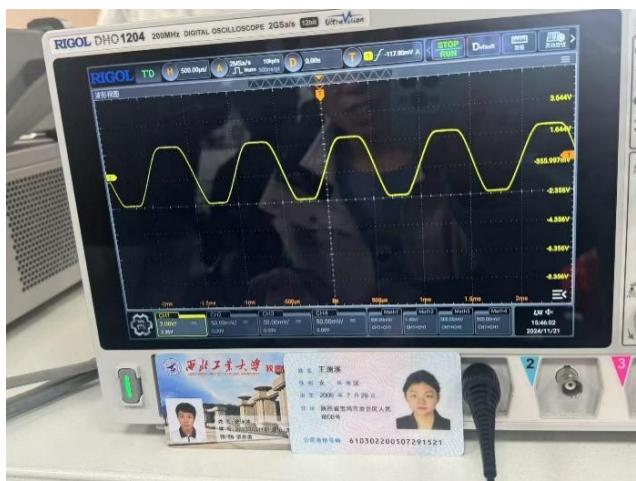
\includegraphics[keepaspectratio]{images/6ad649fc84f56e62492058cfda8b5691a51f16579c6a44ff60ebf20376eb8aaa.jpg}}

\section{（2）测量放大倍数}\label{ux6d4bux91cfux653eux5927ux500dux6570}

①无负载时：

\pandocbounded{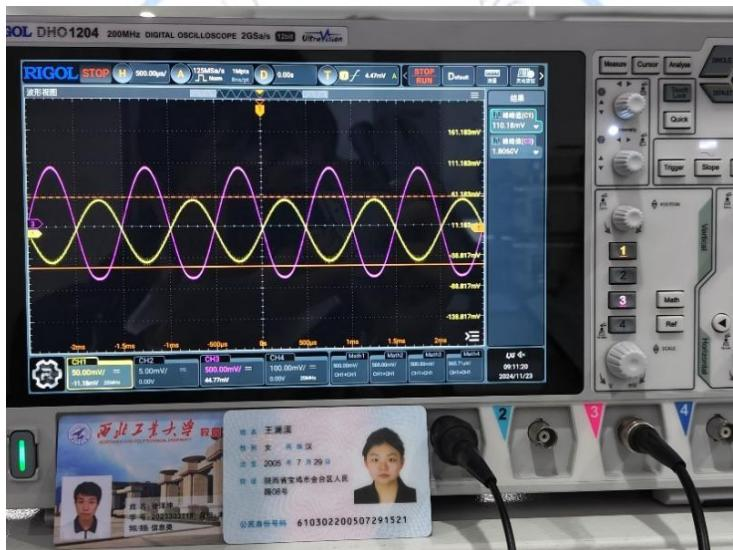
\includegraphics[keepaspectratio]{images/e5d6a048ec469ca23ffd0215321323791d708a06b91a1a3eab15fcb8c601cfe7.jpg}}

由示波器读数可知: \(V_{i} = 110.10 m V, V_{o} = 1.806 V\) ,
则空载放大倍数:

\[
A _ {V 1} = \frac {V _ {o}}{V _ {i}} = \frac {1 . 8 0 6 V}{1 1 0 . 1 8 m V} = 1 6. 3 9
\]

② 有负载（ \(R_{L} = 2k\Omega\) ）时：

\pandocbounded{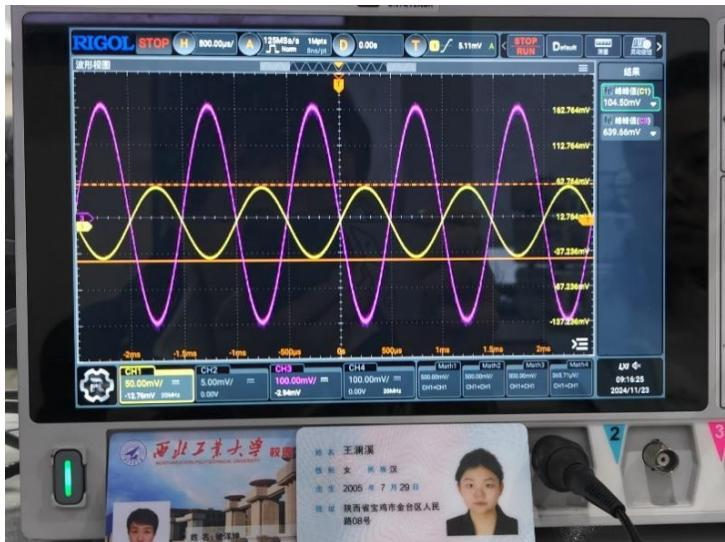
\includegraphics[keepaspectratio]{images/cd3bbc356bb98af421f40a9d1a770aa46819d35184d6024f8bbc5e094bf6d07d.jpg}}

由示波器读数可知:
\(V_{i} = 104.50 \mathrm{~mV}, V_{o} = 639.66 \mathrm{~mV}\) ,
则有载放大倍数:

\[
A _ {V 2} = \frac {V _ {o}}{V _ {i}} = \frac {6 3 9 . 6 6 m V}{1 0 4 . 5 m V} = 6. 1 2
\]

\section{（3）测量输入输出电阻}\label{ux6d4bux91cfux8f93ux5165ux8f93ux51faux7535ux963b}

\section{① 测量输入电阻：}\label{ux6d4bux91cfux8f93ux5165ux7535ux963b}

在输入端，接入电阻 \(R = 1 k \Omega\) ，测量电阻 R 两端的对地电位
\(V_{s}\) 和 \(V_{i}\) ，如图

\pandocbounded{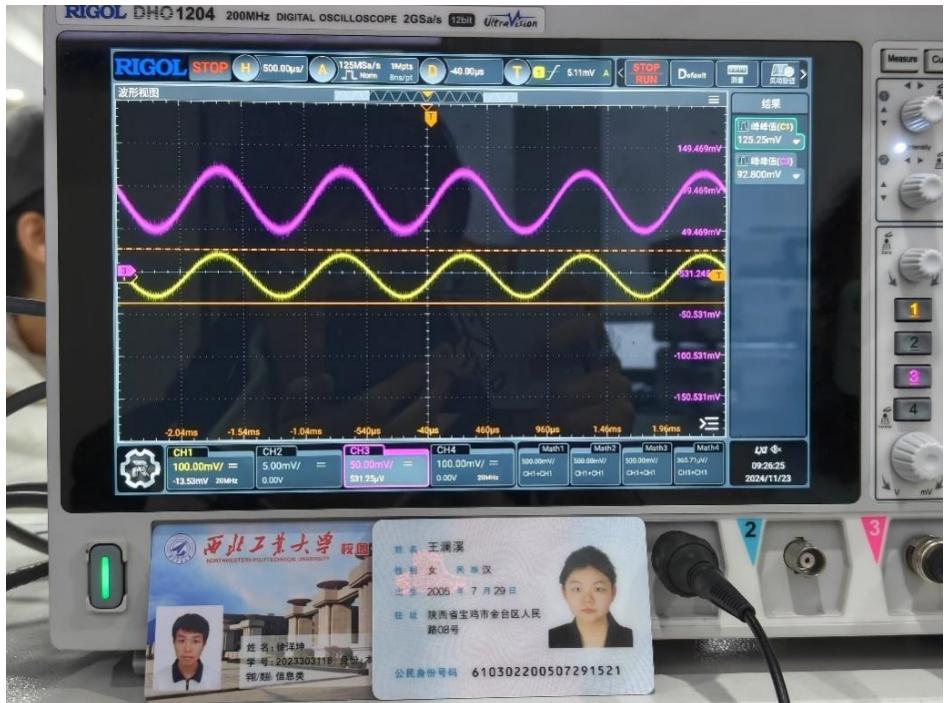
\includegraphics[keepaspectratio]{images/63805bb9c20848925a6829de75d085bf08b3a3cdb378f761cde7f628a08113da.jpg}}

由示波器读数得 \(V_{s} = 125.25mV\) ， \(V_{i} = 92.8mV\)
，代入公式可得：

\[
R _ {i} = \frac {V _ {i}}{V _ {s} - V _ {i}} R = \frac {9 2 . 8}{1 2 5 . 2 5 - 9 2 . 8} \cdot 1 k \Omega = 2. 8 6 k \Omega
\]

\section{②测量输出电阻：}\label{ux6d4bux91cfux8f93ux51faux7535ux963b}

空载时的输出电压 \(V_{o}\)

\pandocbounded{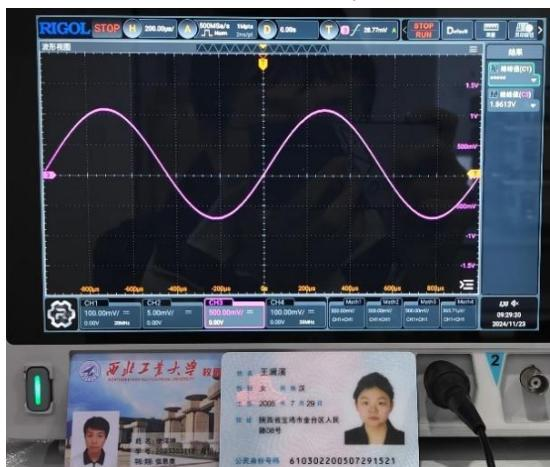
\includegraphics[keepaspectratio]{images/0ba3cbff4d30c496c6fe1bc1637f17a3035812bb4024830c7a6bf1e8dab07221.jpg}}

带负载 \(R_{L} = 2 k \Omega\) 后的输出电压 \(V_{L}\)

\pandocbounded{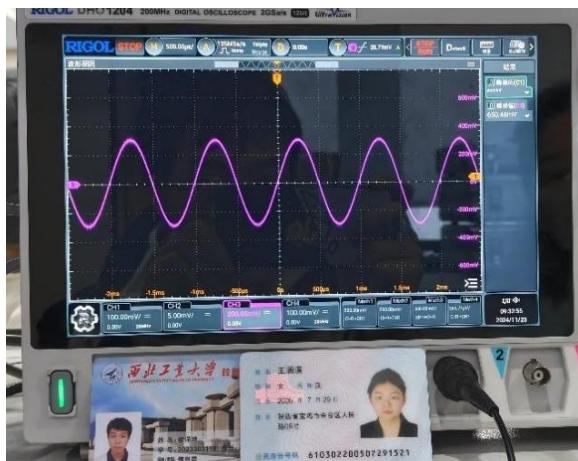
\includegraphics[keepaspectratio]{images/63bd4435f4e1616903148ac34b69a7d4ab9f6afbcfa039177989c32c2b2ecdca.jpg}}

由示波器读数得 \(V_{o} = 1.8613 V, V_{L} = 650.48 m V\) , 代入公式可得:

\[
R _ {o} = \left(\frac {V _ {o}}{V _ {L}} - 1\right) R _ {L} = \left(\frac {1 . 8 6 1 3}{0 . 6 5 0 4 8} - 1\right) \cdot 2 k \Omega = 3. 7 2 3 k \Omega
\]

\section{（4）测量幅频特性}\label{ux6d4bux91cfux5e45ux9891ux7279ux6027}

保持输入信号幅度不变，改变频率，先测量中频段（选取 \(1\mathrm{kHz}\)
）时的输出电压：

\pandocbounded{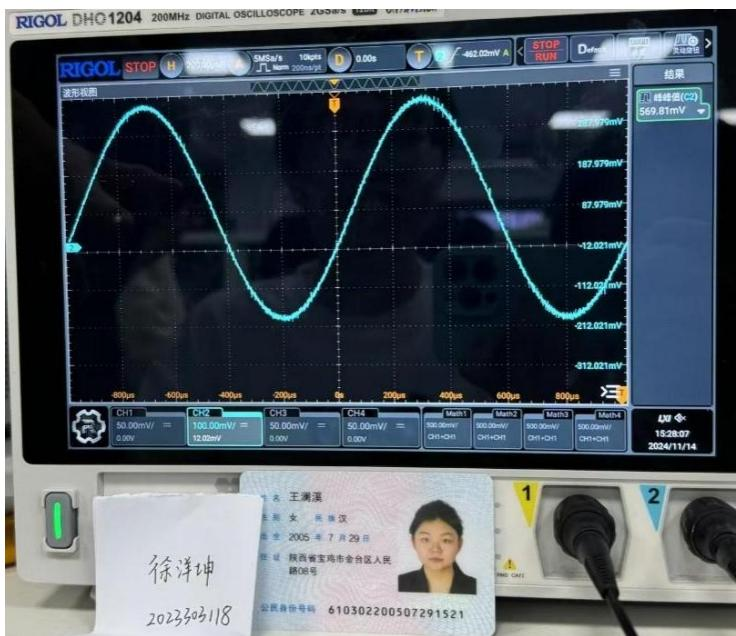
\includegraphics[keepaspectratio]{images/88de03e302b09b59921d21abf741c1d6aef25a28a7bad1929222d39d781d3847.jpg}}

由示波器读数得 \(u_{o} = 569.81 \mathrm{~mV}\) , 计算
\(u_{L} = u_{H} = 0.707 u_{o} = 402 \mathrm{~mV}\) , 调整输入信号频率,
使得输出电压降至 \(400 \mathrm{mV}\) 左右:

\pandocbounded{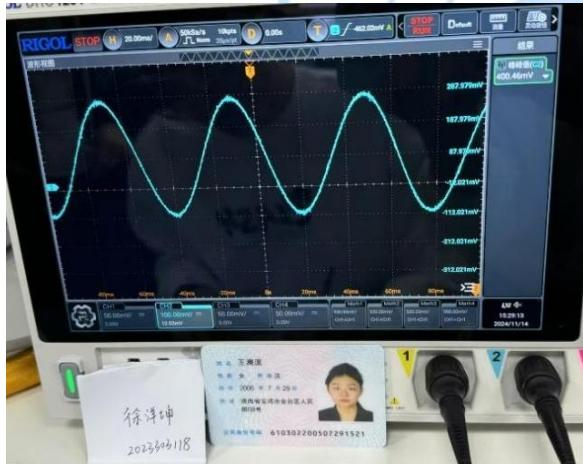
\includegraphics[keepaspectratio]{images/7ff1fd3685c574f205a883f2ba7329e5ea441513f9daa9978d3cca51879a2f31.jpg}}

\pandocbounded{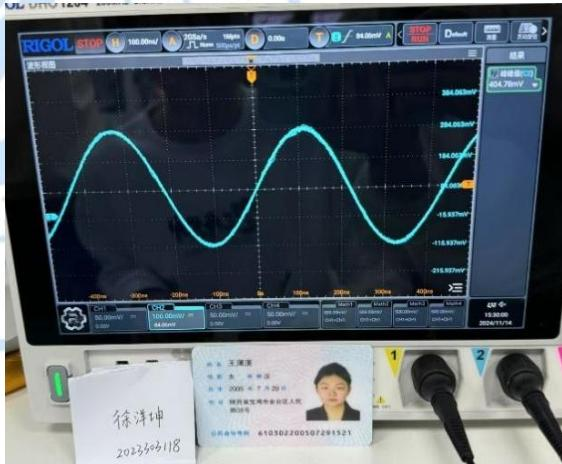
\includegraphics[keepaspectratio]{images/dcbb2a8f0efac11eaf411b8660289f5cdf4511205880fe3af151f86238473f28.jpg}}

记录此时信号的低频频率和高频频率即为下限额率 \(f_{L} = 16 \mathrm{~Hz}\)
上限频率 \(f_{H} = 1.92 \mathrm{MHz}\) 即可由此计算同频带
\(f_{BW} = f_{H} - f_{L}\) 。

\section{六、结论与分析}\label{ux516dux7ed3ux8bbaux4e0eux5206ux6790}

\begin{enumerate}
\def\labelenumi{\arabic{enumi}.}
\tightlist
\item
  数据分析：通过使用Multisim软件进行模拟仿真，将得到的放大倍数、输入输出电阻、频率特性参数与本实验实际测得的数据进行对比，其近似程度较大，在合理范围内。\\
\item
  实验分析：由上述实验的得出的结果可知，实验误差较小，故可基本认为实验值与计算值相等。\\
\item
  实际误差讨论：寻找静态工作点时，观察示波器调试到临界失真条件时，不能很好的掌握波形输出恰好在临界点导致测量的输出电压与理论值有误差，在操作时应尽量多调试几次找到波形最合适的点。
\end{enumerate}

在测量幅频特性中,测出中频带输出电压 \(u_{o}\)
后，调整输入信号频率时，很难严格使输出信号等于 \(0.707 u_{o}\)
，只能尽可能保证接近，应多次细化调整，降低误差。

\section{实验三、运算放大器类型与主要指标}\label{ux5b9eux9a8cux4e09ux8fd0ux7b97ux653eux5927ux5668ux7c7bux578bux4e0eux4e3bux8981ux6307ux6807}

\section{一、实验目的}\label{ux4e00ux5b9eux9a8cux76eeux7684-1}

\begin{enumerate}
\def\labelenumi{\arabic{enumi}.}
\tightlist
\item
  查阅芯片LM324,OP07两种运放的规格书。\\
\item
  制作两种芯片构成的电压缓冲器电路，测量寻失调电压与共模输入范围。\\
  3.测试LM324构成的电压缓冲器电路的幅频特性。
\end{enumerate}

\section{二、实验原理}\label{ux4e8cux5b9eux9a8cux539fux7406-1}

1.两种芯片的规格书

\begin{longtable}[]{@{}llllll@{}}
\toprule\noalign{}
\endhead
\bottomrule\noalign{}
\endlastfoot
& \multicolumn{3}{l}{%
LM324} & \multicolumn{2}{l@{}}{%
OP07} \\
\multirow{2}{*}{电源电压范围(V)} & LM324B/LM324BA & \multicolumn{2}{l}{%
MAX 40} & 单电源 & MAX 44V \\
& LM324XX & \multicolumn{2}{l}{%
MAX 32} & 双电源 & MAX ±22V \\
\multirow{2}{*}{失调电压(V)} & LM324B & TYP±0.6m & MAX ±3m & OP07C &
TYP±60μ \\
& LM324BA & TYP±0.3m & MAX±2m & OP07D & MAX±150μ \\
\multirow{3}{*}{开环增益(mV)} & \multicolumn{3}{l}{%
\multirow{3}{*}{MIN 50,TYP 100(Vs=15V,Vo=1\textasciitilde11V, Rl≥10kΩ)}}
& OP07C & MIN 100 TYP 100 \\
& & & & OP07D & TYP 400 \\
& & & & \multicolumn{2}{l@{}}{%
1.4V\textless Vo\textless11.4V, Rl=500kΩ} \\
\multirow{4}{*}{压摆率(V)} & \multirow{3}{*}{V+} & Io=-50μA & TYP 1.35
MAX 1.5 & \multicolumn{2}{l@{}}{%
\multirow{4}{*}{MIN ±11.5 TYP±12.8}} \\
& & Io=-1mA & TYP 1.4 MAX 1.6 \\
& & Io=-5mA & TYP 1.5 MAX 1.75 \\
& V- & Io=-50μA & TYP 0.1 MAX 0.15 \\
共模输入范围 & \multicolumn{3}{l}{%
MIN V- MAX -1.5V} & \multicolumn{2}{l@{}}{%
MIN±13V TYP±14V} \\
\end{longtable}

\begin{enumerate}
\def\labelenumi{\arabic{enumi}.}
\setcounter{enumi}{1}
\tightlist
\item
  电压缓冲器电路图：
\end{enumerate}

\pandocbounded{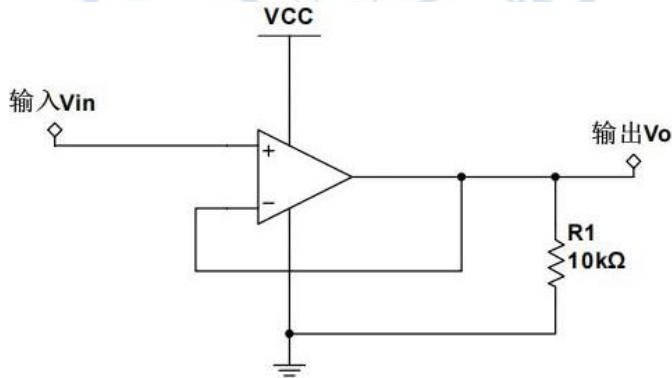
\includegraphics[keepaspectratio]{images/32db693d697e983ce83114dd7236208deaa65518457e9aab188becdb342ad14b.jpg}}\\
图1 电压缓冲器

3.失调电压：

在实际的运算放大器中，当两个输入端电压完全相同时，输出端并不为零，而是有一个小的非零电压。为了使输出端电压为零，必须在输入端施加一个小的差分电压，这个电压称为输入失调电压
\(\mathrm{V_{OS}}\)
，可以看作是一个与运算放大器的反相输入端串联的电压源。对于理想运算放大器，失调电压为0。

4.共模输入范围：

共模输入范围是指运算放大器能够正常工作的输入电压范围。在这个范围内，输入信号的共模部分（即两个输入端电压的平均值）可以变化，而不会导致运算放大器的性能显著下降。

\section{三、实验内容}\label{ux4e09ux5b9eux9a8cux5185ux5bb9-1}

1.分别测量由LM324与OP07运放芯片的失调电压；\\
2.搭建电压缓冲器电路，分别测试由LM324与OP07两种运放芯片构成的缓冲器电路的共模输入范围；\\
3.测试LM324构成的电压缓冲器电路的幅频特性。

\section{四、实验电路方案}\label{ux56dbux5b9eux9a8cux7535ux8defux65b9ux6848-1}

\pandocbounded{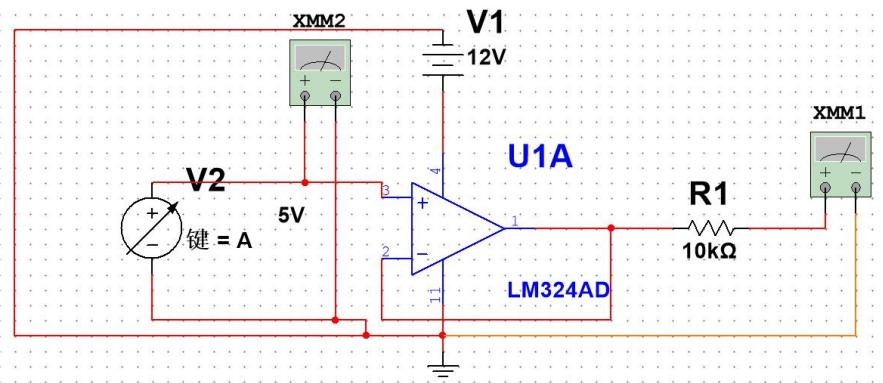
\includegraphics[keepaspectratio]{images/70c92920e7e145cb5eea11f0e718574449ef0eba8e04bef2ed4b5eface411d8c.jpg}}\\
图2理论仿真电路（LM324版）

\section{五、测试与数据记录}\label{ux4e94ux6d4bux8bd5ux4e0eux6570ux636eux8bb0ux5f55-1}

\section{1. 测试用仪器}\label{ux6d4bux8bd5ux7528ux4eeaux5668-1}

直流稳压；示波器；信号发生器；LM324；OP07；10kΩ电阻；导线若干。

\section{2. 实验步骤}\label{ux5b9eux9a8cux6b65ux9aa4-1}

\section{（1）测量运放失调电压：}\label{ux6d4bux91cfux8fd0ux653eux5931ux8c03ux7535ux538b}

①制作图1所示的电压缓冲器，输出接 \(10 \mathrm{k} \Omega\) 负载，单电源
\(12 \mathrm{~V}\) 供电。\\
(2) 使用 LM324 运放, 在输入端 \(\mathrm{V}_{\mathrm{in}}\) 增加
\(0 \mathrm{~V}\) 到 \(12 \mathrm{~V}\) 的直流电压, 所用值自定,
保证运放正常工作,
使得输出几乎等于输入实现电压跟随。测试运放正负输入端电压差即为失调电压,
记为 \(\mathrm{V}_{1}\) 。\\
(3)换成高精度运放 OP07, 使用以上相同条件进行测试 OP07 失调电压, 记为
\(\mathrm{V}_{2}\) , 观察两者区别, 以及是否符合各自规格书指标。

\section{（2）测量共模输入范围：}\label{ux6d4bux91cfux5171ux6a21ux8f93ux5165ux8303ux56f4}

使用LM324构成的电压缓冲器电路，改变输入电压 \(V_{i}\)
从0V升高到电源电压，测量输出电压 \(V_{o}\) ，对比 \(V_{i}\) 与 \(V_{o}\)
。当 \(V_{i} \leq u_{cm}\) 时，如果 \(V_{i} = V_{o}\)
，则处于电压跟随状态，在共模输入范围内；持续增大 \(V_{i}\) 后，当增大至
\(V_{i} > u_{cm}\) 时，如果 \(V_{i} \neq V_{o}\)
，则电压跟随状态消失，超出了共模输入范围， \(u_{cm}\)
即为共模输入电压最大值，共模输入范围即为 \(0 \leq V_{i} \leq u_{cm}\) 。

\section{（3）测试电压缓冲器电路的幅频特性}\label{ux6d4bux8bd5ux7535ux538bux7f13ux51b2ux5668ux7535ux8defux7684ux5e45ux9891ux7279ux6027}

使用LM324构成的电压缓冲器电路，将输入信号改为信号发生器输入，保持输入信号幅度不变，改变频率。利用示波器观察输出电压，先测量中频段（选取1kHz）时的输出电压；再分别降低、提高频率多次试验，当输出电压下降为中频段的0.707倍时，相对应的低频频率和高频频率即为下限额率
\(f_{L}\) 和上限频率 \(f_{H}\) ，并由此计算通频带
\(f_{BW} = f_{H} - f_{L}\) 。

\section{3.
实验结果与数据记录}\label{ux5b9eux9a8cux7ed3ux679cux4e0eux6570ux636eux8bb0ux5f55-1}

\section{（1）测量运放失调电压：}\label{ux6d4bux91cfux8fd0ux653eux5931ux8c03ux7535ux538b-1}

\pandocbounded{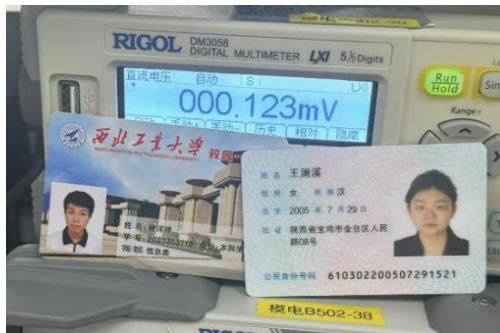
\includegraphics[keepaspectratio]{images/4b95219fede83eed76dad7d8223197dc14df5026d6ae57cb8cfa684d9690bcd5.jpg}}\\
图3LM324运放失调电压

\pandocbounded{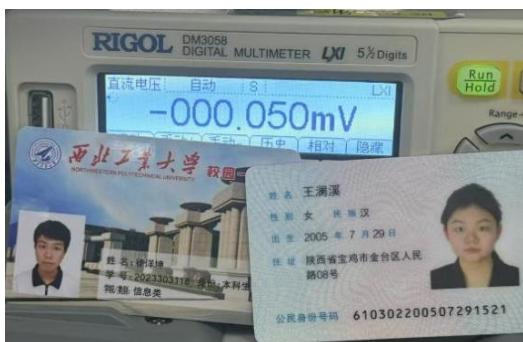
\includegraphics[keepaspectratio]{images/0a4b9796de5ef3bdcf945cc2e09ba32d70055499194073f1ebb07e80a01a160d.jpg}}\\
图4OP07运放失调电压

即 \(\mathrm{LM324}\) 运放失调电压:
\(V_{\mathrm{OS}} = 0.123 \mathrm{mV}\) ; \(\mathrm{OP07}\)
运放失调电压: \(V_{\mathrm{OS}} = 50 \mu \mathrm{V}\) 。

\section{（2）测量共模输入范围：}\label{ux6d4bux91cfux5171ux6a21ux8f93ux5165ux8303ux56f4-1}

记录电压跟随的最大值即恰好不发生电压跟随的临界值

\pandocbounded{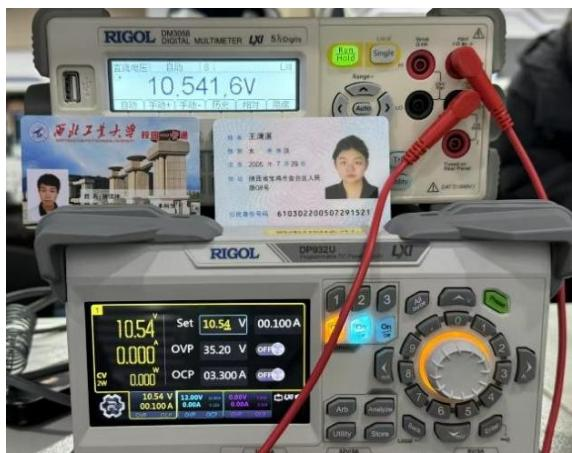
\includegraphics[keepaspectratio]{images/43ea6ed4b80ef85648abee5a33568cbf8ba7082cb515859f5c0c279bbba7bb33.jpg}}\\
图5电压跟随最大值图

\pandocbounded{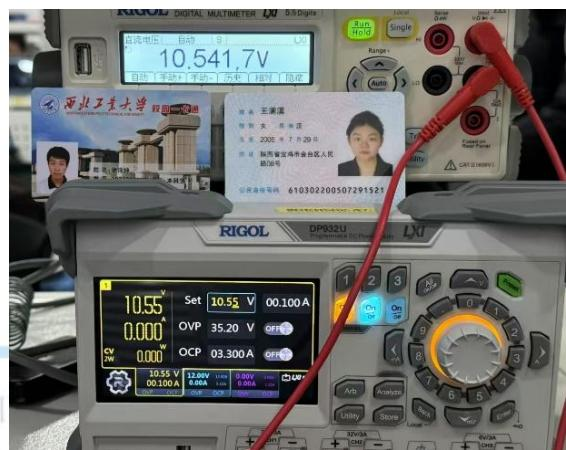
\includegraphics[keepaspectratio]{images/c3181a833c6dd02d1673a7826af1e2a45ddd8e40701a311d2693e8a651b6c5b2.jpg}}\\
图6恰好不发生电压跟随

由实验结果, 当 \(V_{i} \leq 10.54 V\) 时, \(V_{i} = V_{o}\) ,
处于电压跟随状态, 在共模输入范围内;

当增大至 \(V_{i} = 10.55 V > 10.54 V\) 时,
\(V_{o} = 10.54 V \neq V_{i}\) , 电压跟随状态消失, 超出了共模输入范围,
则共模输入范围即为 \(0 \leq V_{i} \leq 10.54 V\) 。

\section{（3）测试电压缓冲器电路的幅频特性}\label{ux6d4bux8bd5ux7535ux538bux7f13ux51b2ux5668ux7535ux8defux7684ux5e45ux9891ux7279ux6027-1}

保持输入信号幅度不变，改变频率，先测量中频段（选取 \(1\mathrm{kHz}\)
）时的输出电压：

①由示波器读数得 \(u_{o} = 208.84mV\) ，计算 \(0.707u_{o} = 147.672mV\)
，调整输入信号频率，使得输出电压降至 \(147\mathrm{mV}\) 左右：\\
②当降低输入信号频率至 \(1 \mathrm{~Hz}\) 时, \(u_{o} = 213 m V\)
依旧未发生下降, 故 LM324 运放构成的电压缓冲器对直流信号仍有正常功能,
下限截止频率 \(f_{L} = 0 \mathrm{~Hz}\) 。\\
③当提高输入信号频率至 \(1.4 \mathrm{MHz}\) 时, \(u_{o} = 138.8 m V\) ,
接近 \(147 \mathrm{mV}\) , 可得上限截止频率 \(f_{H} = 1.4 \mathrm{MHz}\)
。

由此计算通频带 \(f_{BW} = f_{H} - f_{L} = 1.4MHz\)

\pandocbounded{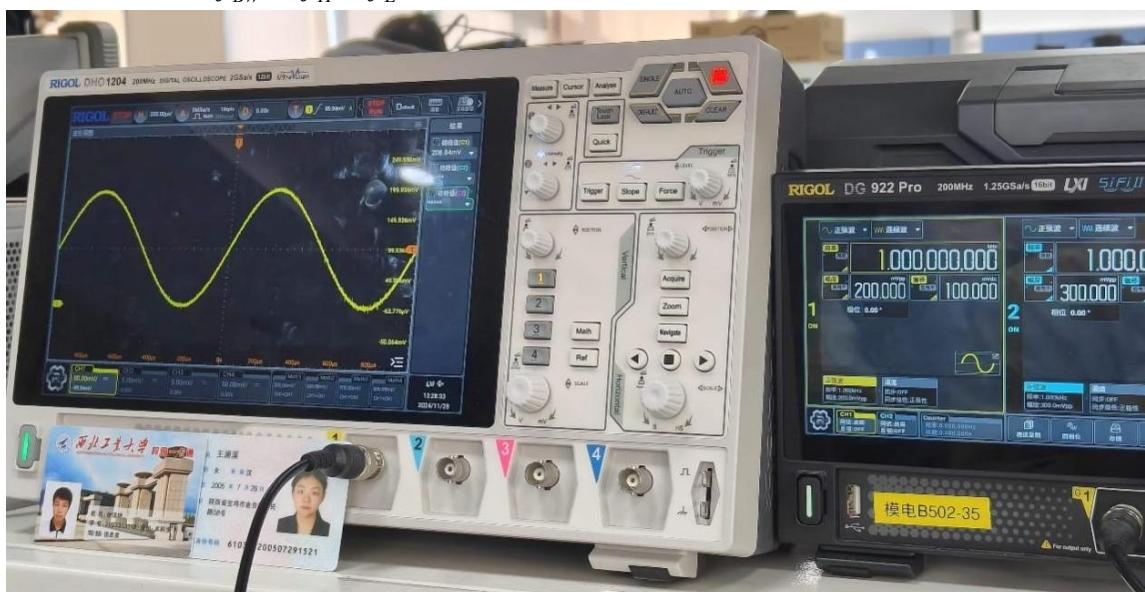
\includegraphics[keepaspectratio]{images/1b4b0b5c9fb84887a80298d8a875591f3a2f5489ff5fef4121e0dd41710281db.jpg}}\\
图7中频段输出电压

\pandocbounded{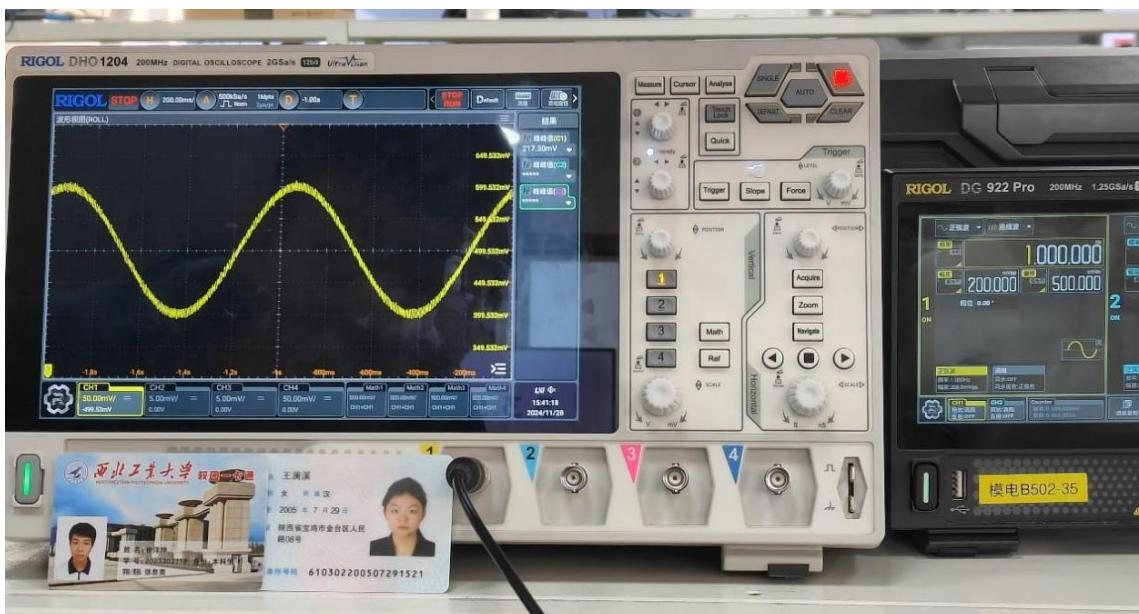
\includegraphics[keepaspectratio]{images/25d194e5efe781d975870d0d63b295429f08d2bfe3baf8af7eefa4fba400ad65.jpg}}\\
图8低频段输出电压

\pandocbounded{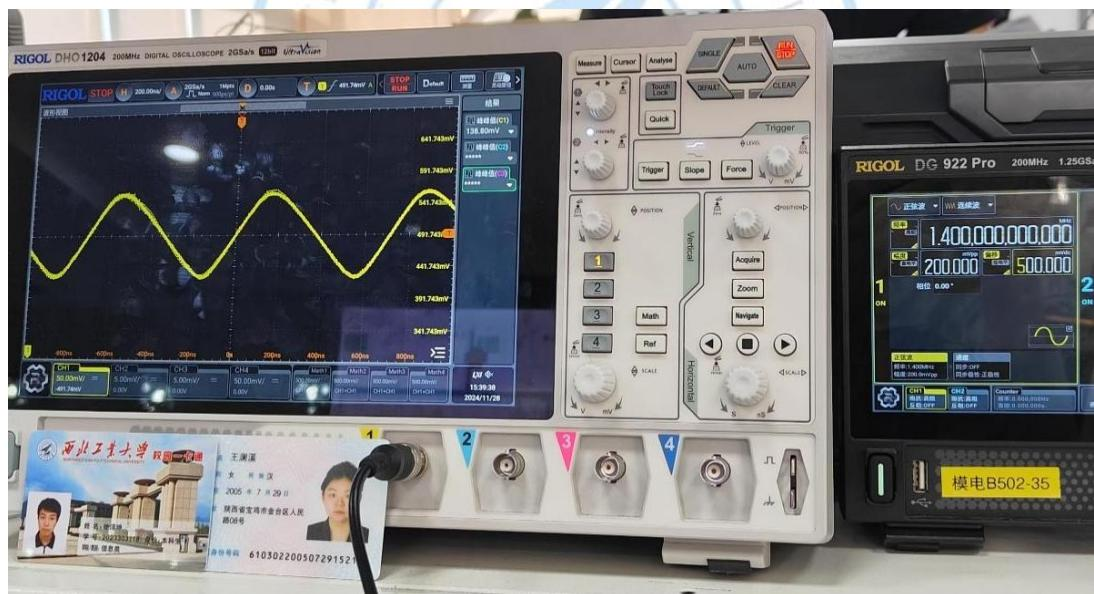
\includegraphics[keepaspectratio]{images/218607582c8f79e6f27395a3ff6cf4bf19cf615c90942eeb6828e9fdbd95cf9e.jpg}}\\
图9高频段输出电压

\section{六、结论与分析}\label{ux516dux7ed3ux8bbaux4e0eux5206ux6790-1}

\begin{enumerate}
\def\labelenumi{\arabic{enumi}.}
\tightlist
\item
  数据分析: 本验测得 LM324 运放失调电压:
  \(V_{\mathrm{OS}} = 0.123 \mathrm{mV}\) ; OP07 运放失调电压:
  \(V_{\mathrm{OS}} = 50 \mu \mathrm{V}\) 。LM324
  构成的电压缓冲器共模输入范围为 \(0 \leq V_{i} \leq 10.54 V\) ,
  下限截止频率 \(f_{L} = 0 \mathrm{~Hz}\) , 上限截止频率
  \(f_{H} = 1.4 \mathrm{MHz}\) , 均在芯片规格书的合理误差范围内。\\
\item
  实验分析：由上述实验的得出的结果可知，实验误差较小，故可基本认为真实值与计算值相等。\\
\item
  实际误差讨论：在测量幅频特性中，测出中频带输出电压 \(u_{o}\)
  后，调整输入信号频率时，很难严格使输出信号等于 \(0.707 u_{o}\)
  ，只能尽可能保证接近，应多次细化调整，降低误差。
\end{enumerate}

\section{实验四、运算放大器线性应用}\label{ux5b9eux9a8cux56dbux8fd0ux7b97ux653eux5927ux5668ux7ebfux6027ux5e94ux7528}

\section{一、实验目的}\label{ux4e00ux5b9eux9a8cux76eeux7684-2}

\begin{enumerate}
\def\labelenumi{\arabic{enumi}.}
\tightlist
\item
  加深对集成运算放大器的基本应用电路和性能参数的理解。\\
\item
  掌握由集成运算放大器组成的比例、加法、减法、积分和微分等基本运算电路的功能。
\end{enumerate}

\section{二、实验原理}\label{ux4e8cux5b9eux9a8cux539fux7406-2}

\section{1.减法电路}\label{ux51cfux6cd5ux7535ux8def}

减法电路实际上是反相放大电路和同相放大电路的组合，电路图见图1。对于理想运算放大器，该电路的输出电压与输入电压之间的关系为：

\[
V _ {o} = \left(1 + \frac {R _ {f}}{R _ {1}}\right) \left(\frac {R _ {3}}{R _ {2} + R _ {3}}\right) V _ {i 2} - \frac {R _ {f}}{R _ {1}} V _ {i 1}
\]

当 \(R_{1} = R_{2}, R_{3} = R_{f}\) 时

\[
V _ {o} = \frac {R _ {f}}{R _ {1}} \left(V _ {i 2} - V _ {i 1}\right)
\]

\section{2.反相积分电路}\label{ux53cdux76f8ux79efux5206ux7535ux8def}

反相积分电路电路图见图2,对于理想运算放大器，该电路的输出电压与输入电压之间的关系为

\[
V _ {o} (t) = - \frac {1}{R _ {1} C} \int V _ {i} d t + V _ {C} (0)
\]

式中， \(V_{C}(0)\) 是 \(t = 0\) 时刻电容 \(C\) 两端的电压值，即初始值。

如果 \(V_{i}\) 是幅值为 \(E\) 的阶跃电压, 并设 \(V_{C}(0) = 0\) ,
则输出电压 \(V_{o}\) 和时间 \(t\) 成正比, 即

\[
V _ {o} (t) = - \frac {1}{R _ {1} C} \int_ {0} ^ {t} E d t = - \frac {E}{R _ {1} C} t
\]

\section{三、实验内容}\label{ux4e09ux5b9eux9a8cux5185ux5bb9-2}

\section{1.减法电路}\label{ux51cfux6cd5ux7535ux8def-1}

按照图1的减法器电路结构和参数搭建电路，测试输出信号波形以及参数，完成下表：

表 1 减法电路数据表

\begin{longtable}[]{@{}llll@{}}
\toprule\noalign{}
\endhead
\bottomrule\noalign{}
\endlastfoot
\multicolumn{2}{@{}l}{%
ui1pp / mV} & & \\
\multicolumn{2}{@{}l}{%
ui2pp / mV} & & \\
\multicolumn{2}{@{}l}{%
uopp / mV} & & \\
\multirow{3}{*}{AV} & 理论值 & & \\
& 仿真值 & & \\
& 实测值 & & \\
\end{longtable}

\section{2.反相积分电路}\label{ux53cdux76f8ux79efux5206ux7535ux8def-1}

按照图2的反相积分电路结构和参数搭建电路，同时测试输入信号和输出信号波形，观察二者关系。

\section{四、实验电路方案}\label{ux56dbux5b9eux9a8cux7535ux8defux65b9ux6848-2}

本实验两种电路方案模拟图如下图1、图2所示：

\pandocbounded{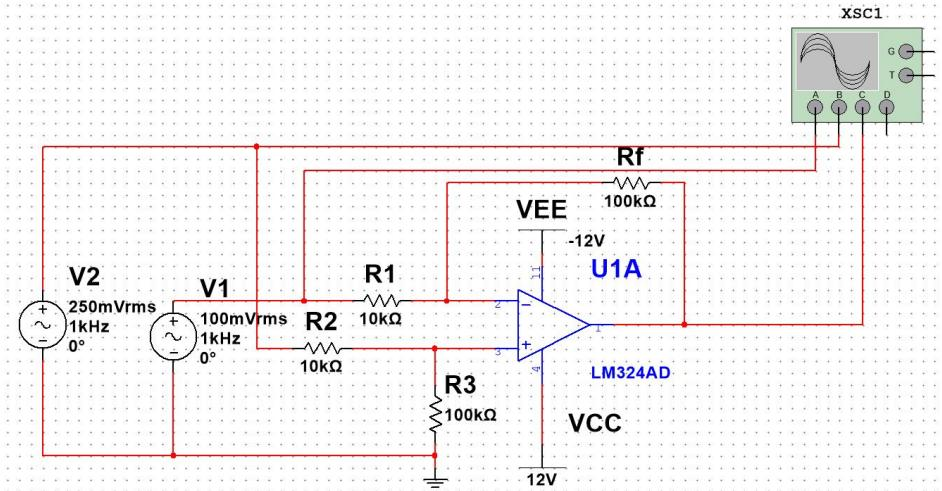
\includegraphics[keepaspectratio]{images/d811c400f4faad119eee7e1b8b281625ac2d09c3339d68be9c86bebc8ba31e6a.jpg}}\\
图1 减法电路

\pandocbounded{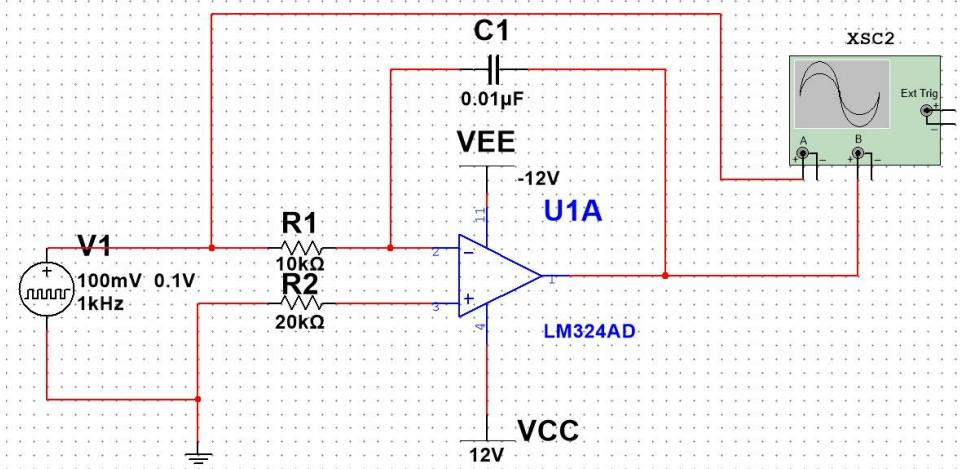
\includegraphics[keepaspectratio]{images/597712d36b38bccf151e46c5debbbd05ea70a71018a5aa0dbc1c28749be78300.jpg}}\\
图2反相积分电路

\section{五、测试与数据记录}\label{ux4e94ux6d4bux8bd5ux4e0eux6570ux636eux8bb0ux5f55-2}

\section{1. 测试用仪器}\label{ux6d4bux8bd5ux7528ux4eeaux5668-2}

LM324 运放芯片,电阻若干, \(0.01 \mu F\) 电容, 函数发生器, 示波器,
直流电源;

\section{2.实验步骤}\label{ux5b9eux9a8cux6b65ux9aa4-2}

\section{（1）减法电路}\label{ux51cfux6cd5ux7535ux8def-2}

按图1所示结构参数搭建电路，同相输入端输入峰峰值为 \(250\mathrm{mV}\)
，频率 \(1\mathrm{kHz}\) 正弦波（0偏移）记为 \(V_{i2}\)
，反相输入端输入峰峰值为 \(100\mathrm{mV},1\mathrm{kHz}\)
正弦波（0偏移）记为 \(V_{i1}\)
，调整改变输入信号幅度，继续验证减法电路性质，并完成表1。

\section{（2）反相积分电路}\label{ux53cdux76f8ux79efux5206ux7535ux8def-2}

按图2所示结构参数搭建电路，输入信号为方波，频率 \(1\mathrm{kHz}\)
，高电平 \(100\mathrm{mV}\) ，低电平 \(-100\mathrm{mV}\) ，占空比
\(50\%\)
。示波器同时测试输入信号和输出信号，观察输出信号和输入信号关系。

\section{3. 数据记录}\label{ux6570ux636eux8bb0ux5f55}

\section{（1）减法电路}\label{ux51cfux6cd5ux7535ux8def-3}

同相输入端信号记为 \(V_{i2}\) （蓝色波形），反相输入端信号记为
\(V_{i1}\) （黄色波形），

输出电压为 \(V_{o}\) （紫色波形）

调整 \(V_{i2}, V_{i1}\)
幅度，得到两组数据结果，如图3,图4所示，记录数据填入表2如下；

\pandocbounded{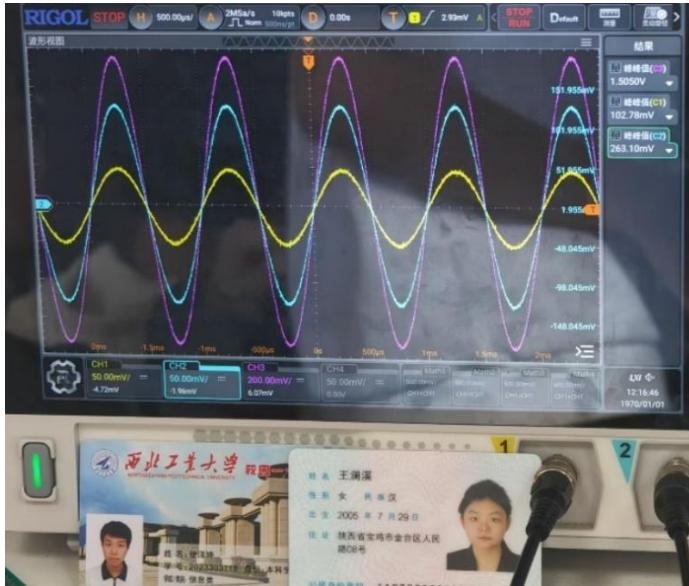
\includegraphics[keepaspectratio]{images/358f04bb990b56b656250bfaadec9ab0f9bfbbc5f8fb63fe7be6905720e676c0.jpg}}\\
图3减法电路波形比较（1）

由示波器读数可知
\(V_{i2} = 263.1 m V, V_{i1} = 102.78 m V, V_{o} = 1.505 V\)

计算差模信号放大倍数
\(A_{V} = \frac{1.505 V}{(263.1 - 102.78) m V} = 9.387\)

再更换调整输入信号幅度，进一步验证：

\pandocbounded{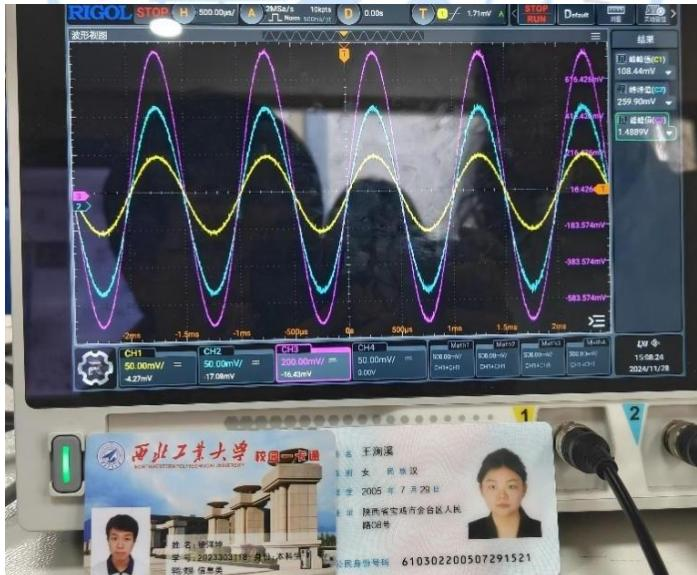
\includegraphics[keepaspectratio]{images/ad09467cd12f76cef6dc19d2c43aa1083e3804b07da3be547e25460447ec92ad.jpg}}\\
图4减法电路波形比较（2）

由示波器读数可知
\(V_{i2} = 108.44 \mathrm{~mV}, V_{i1} = 259.9 \mathrm{~mV}, V_{o} = 1.4889 \mathrm{~V}\)

计算差模信号放大倍数
\(A_{V} = \frac{1.4889 V}{(259.9 - 108.44) m V} = 9.83\)

两组数据 \(A_{V 1} = 9.387\) , \(A_{V 2} = 9.83\) ;

对比理论值
\(A_{V} = \frac{R_{f}}{R_{1}} = \frac{100 k \Omega}{10 k \Omega} = 10\)

基本符合减法电路结果预测，满足
\(V_{o} = \frac{R_{f}}{R_{1}} (V_{i2} - V_{i1})\)
，实现输入信号相减后输出。

再使用Multisim软件进行仿真实验，计算 \(A_{V}\) 。

记录上述所有数据，填入表2中如下：

表 2 减法电路数据表

\begin{longtable}[]{@{}llll@{}}
\toprule\noalign{}
\endhead
\bottomrule\noalign{}
\endlastfoot
\multicolumn{2}{@{}l}{%
ui1pp / mV} & 263.1 & 259.9 \\
\multicolumn{2}{@{}l}{%
ui2pp / mV} & 102.78 & 108.44 \\
\multicolumn{2}{@{}l}{%
uopp / mV} & 1505 & 1488.9 \\
\multirow{3}{*}{AV} & 理论值 & 10 & 10 \\
& 仿真值 & 10.022 & 9.991 \\
& 实测值 & 9.378 & 9.83 \\
\end{longtable}

\section{（2）反相积分电路}\label{ux53cdux76f8ux79efux5206ux7535ux8def-3}

记输入电压为 \(V_{i}\) （黄色波形），输出电压为 \(V_{o}\)
（蓝色波形），实验结果如图 5 所示：

\pandocbounded{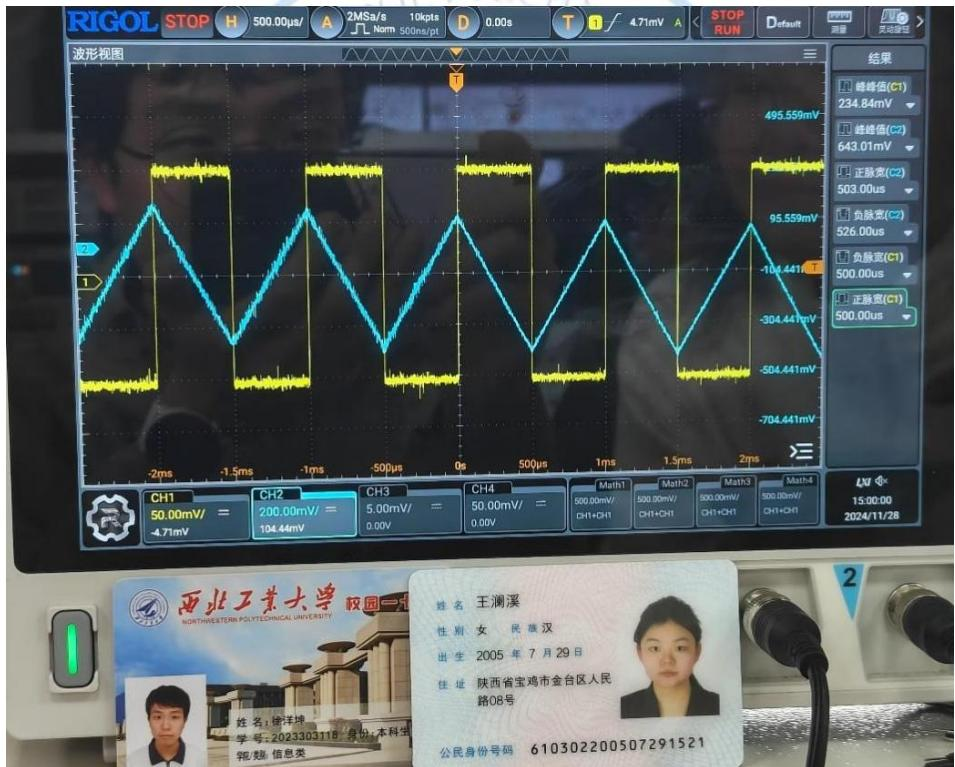
\includegraphics[keepaspectratio]{images/ed58bfd83b0c77b70f153fd8be349030917feb094fa8c29c322a6c379396004d.jpg}}\\
图5反相积分电路

可见，当输入信号 \(V_{i}\) 为方波时，输出信号 \(V_{o}\)
为三角波，且两者满足相位相反关系：

即 \(V_{o}(t) = -\frac{1}{R_{1}C}\int V_{i}dt + V_{C}(0)\)
，满足反相积分电路运算性质。

\section{六、结论与分析}\label{ux516dux7ed3ux8bbaux4e0eux5206ux6790-2}

\begin{enumerate}
\def\labelenumi{\arabic{enumi}.}
\tightlist
\item
  数据分析：验证减法电路性质时，输入输出信号满足的关系，以及利用测量结果计算所得到的
  \(A_{V}\) 与理论值的误差较小，在合理范围内。\\
\item
  实验分析：由上述实验的得出的结果可知，实验误差较小，故可基本认为实验值与真实值相等，电路功能验证有效。\\
\item
  实际误差讨论：由于输入信号幅度较小，波形带有毛刺（不光滑），导致示波器自动测量峰峰值时受一定影响存在误差，但据此计算的结果误差依旧较小；为了降低实验误差，可以在其他条件不变时，增大输入信号幅度，多次测量计算。
\end{enumerate}

\section{实验五、正弦波振荡电路}\label{ux5b9eux9a8cux4e94ux6b63ux5f26ux6ce2ux632fux8361ux7535ux8def}

\section{一、实验目的}\label{ux4e00ux5b9eux9a8cux76eeux7684-3}

1.了解RC正弦波振荡器的工作原理；\\
2.学习正弦波振荡器的电路元件参数选择；\\
3. 学习使用示波器单次触发功能（single）；

\section{二、实验原理}\label{ux4e8cux5b9eux9a8cux539fux7406-3}

1.选频网络的振荡电路：

振荡电路的振荡频率 \(f_0\)
由相位平衡条件(正反馈的电压与输出电压同相位)决定。一个正弦波振荡电路只在一个频率下满足相位平衡条件,
这个频率就是 \(f\) 这就要求在环路中包含一个具有选频特性的网络,
简称选频网络。它可以用 R,C 元件组成也可用 L,C 元件组成。用 R,C
元件组成选频网络的振荡电路称为 RC 振荡电路, 又称为文氏电桥振荡电路,
一般用来产生 \(1\mathrm{Hz} \sim 1\mathrm{MHz}\) 范围内的低频信号; 而用
L,C 元件组成选频网络的振荡电路称为 LC 振荡电路, 一般用来产生
\(1\mathrm{MHz}\) 以上的高频信号。

当放大电路中引入正反馈时，性能就不稳定，会产生自激，从而产生持续的振荡，由直流电变为交流电。欲使振荡电路能自行建立振荡，就必须满足产生振荡的振幅条件和相位条件。这样，在接通电源后，由于电路中存在噪声，它的频谱分布很广，其中也包括
\(\mathrm{f}_0\)
这样一个频率成分。这种微弱的信号，经过放大，通过正反馈的选频网络，使输出幅度愈来愈大，振荡电路自行起振，或者说自激，最后受电路中非线性元件的限制，使振荡幅度自动稳定，趋于稳态平衡，此时
\(\mathrm{Av} = 3\) 。

2.RC桥式振荡电路：

RC桥式振荡电路由两部分组成，即放大电路和选频网络，如图1.1所示。图中
\(\mathrm{R}_3,\mathrm{R}_4\) ， \(\mathbb{R}_{\mathrm{p}}\)
构成负反馈支路,调节电位器 \(\mathbb{R}_{\mathrm{p}}\)
,可以改变负反馈的深度，以满足振荡的振幅条件和改善波形。
\(\mathrm{R_1,R_2,C_1}\) ， \(C_2\)
组成的串、并联电路构成正反馈支路并兼作选频网络。两个反向并联二极管
\(\mathrm{D}_1,\mathrm{D}_2\) 是利用正向电阻的非线性特性实现稳幅的。要求
\(\mathrm{D}_1,\mathrm{D}_2\)
采用硅管(温度稳定性好)，且特性匹配，这样才能保证输出波形正、负半周对称。
\(\mathbb{R}_4\) 的接入是为了消除二极管非线性的影响，以改善波形失真。

\begin{enumerate}
\def\labelenumi{\arabic{enumi}.}
\setcounter{enumi}{2}
\tightlist
\item
  示波器单次触发使用步骤：
\end{enumerate}

\begin{enumerate}
\def\labelenumi{\arabic{enumi}.}
\tightlist
\item
  触发按键(Trigger), 设置触发通道, 触发形式: 自动, 触发边沿: 上升沿;\\
  （2）设置通道合理的时间格和幅度格。调整纵轴和横轴触发点；\\
\item
  电路恢复不振荡的情况, 按单次触发按键(single), 之后让电路起振,
  只要有经过触发点的波形, 就会自动保留在屏幕中;\\
  (4)如果触发出的波形未完整显示在屏幕中(时间超出屏幕或者幅度超出屏幕),
  调整(2)步, 再次(3)步, 重复, 直至触发出需要测试的完整波形。
\end{enumerate}

\section{三、实验内容}\label{ux4e09ux5b9eux9a8cux5185ux5bb9-3}

(1)调节滑动变阻 \(\mathrm{R_p}\)
，使输出波形从无到有直至不失真。在临界起振、正弦波输出及出现临界失真三种情况下测试波形和数据，完成表格
1.1。\\
(2) 保持其他参数不变, 观察 \(C_1 = C_2 = 0.01 \mathrm{uF}\) 和
\(C_1 = C_2 = 0.02 \mathrm{uF}\) 两种情况下
(输出波形不失真)分别测量输出电压 \(\mathrm{V_o}\) 、反馈电压
\(\mathrm{V_f}\) 的有效值和频率 \(\mathrm{f}\) 。

\section{四、实验电路方案}\label{ux56dbux5b9eux9a8cux7535ux8defux65b9ux6848-3}

\pandocbounded{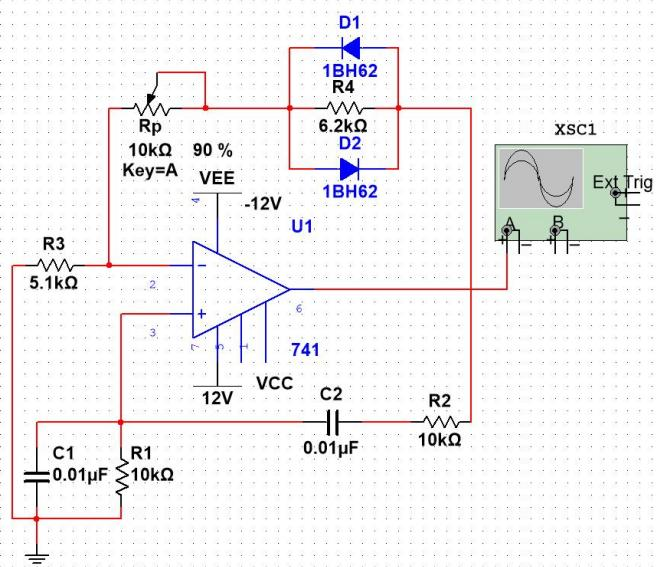
\includegraphics[keepaspectratio]{images/754a6a6b143233a8e5cbd4d2fe848ed05a47b385be6a2c83f83a6cfeccab6059.jpg}}\\
图1.1理论仿真电路

\pandocbounded{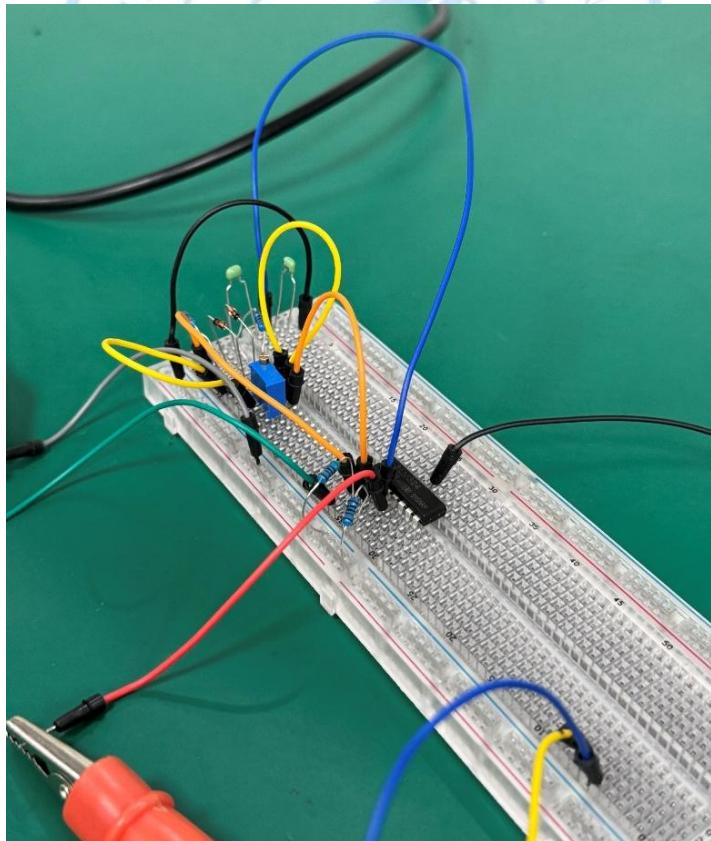
\includegraphics[keepaspectratio]{images/f11e9cb5c08af5598e2673c661c16350a9ac427aea06698c593650487444dd98.jpg}}\\
图1.2 实际连接电路图

\section{五、测试与数据记录}\label{ux4e94ux6d4bux8bd5ux4e0eux6570ux636eux8bb0ux5f55-3}

\section{1. 测试用仪器}\label{ux6d4bux8bd5ux7528ux4eeaux5668-3}

面包板，示波器，741放大器，导线、电阻、二极管、电容若干。

\section{2. 实验步骤}\label{ux5b9eux9a8cux6b65ux9aa4-3}

任务一 接通电源用示波器观察有无正弦波输出

(1)调节滑动变阻 \(\mathrm{R_p}\) , 使输出波形从无到有直至不失真\\
(2)记录临界起振、正弦波输出及出现临界失真情况下的 \(\mathrm{R_p}\) 值\\
(3)分析负反馈强弱对起振条件和输出波形的影响

(4)记录三种情况下(临界起振、正弦波输出及出现临界失真)的输出电压
\(V_{0}\) 。

任务二 测量输出电压 \(\mathrm{V_o}\)

保持其他参数不变，观察 \(\mathrm{C_1 = C_2 = 0.01uF}\) 和
\(\mathrm{C_1 = C_2 = 0.02uF}\)
两种情况下(输出波形不失真)，分别测量输出电压 \(\mathbf{V}_{\circ}\)
、反馈电压 \(\mathrm{V_f}\) 的有效值和频率f

\section{3. 数据记录}\label{ux6570ux636eux8bb0ux5f55-1}

（1）三种情况下的测试波形

A. 临界起振（示波器单次触发抓取）

\pandocbounded{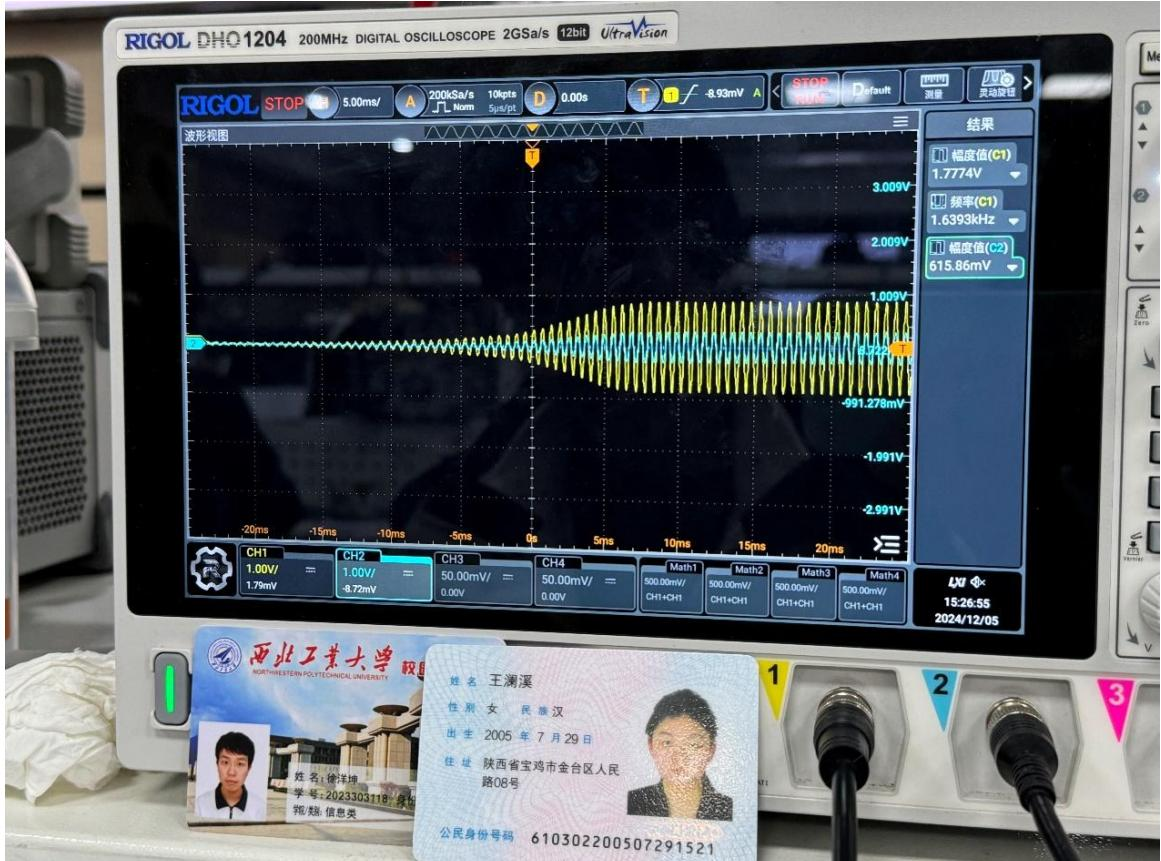
\includegraphics[keepaspectratio]{images/d12060a25b784e063a3a843c7d31d40e49fe724d42f42ea2beec581dfcd3061c.jpg}}

B. 正弦波输出（振幅最大且不失真）

\pandocbounded{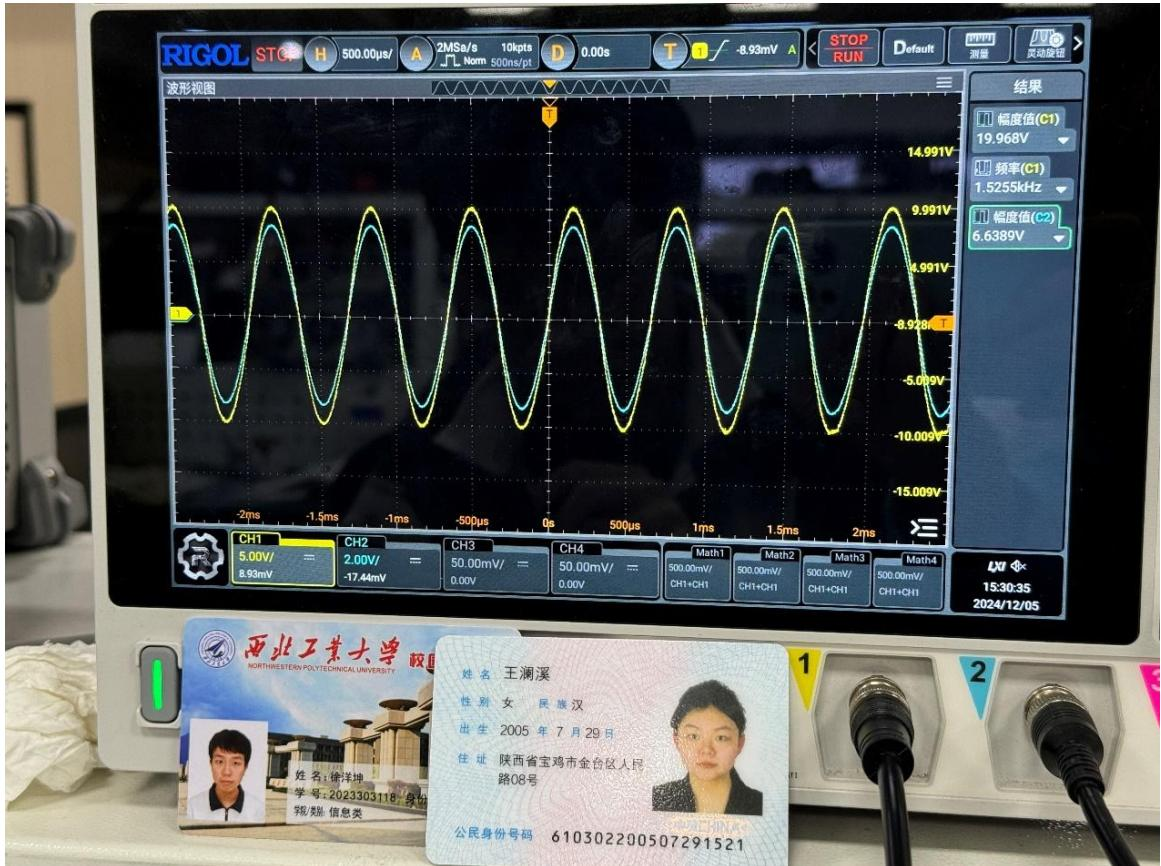
\includegraphics[keepaspectratio]{images/c82712a77ee0809374ec0848fc3c3674da3dea443a3dffd81168a12b6570bf2d.jpg}}\\
C. 临界失真（输出已失真）

\pandocbounded{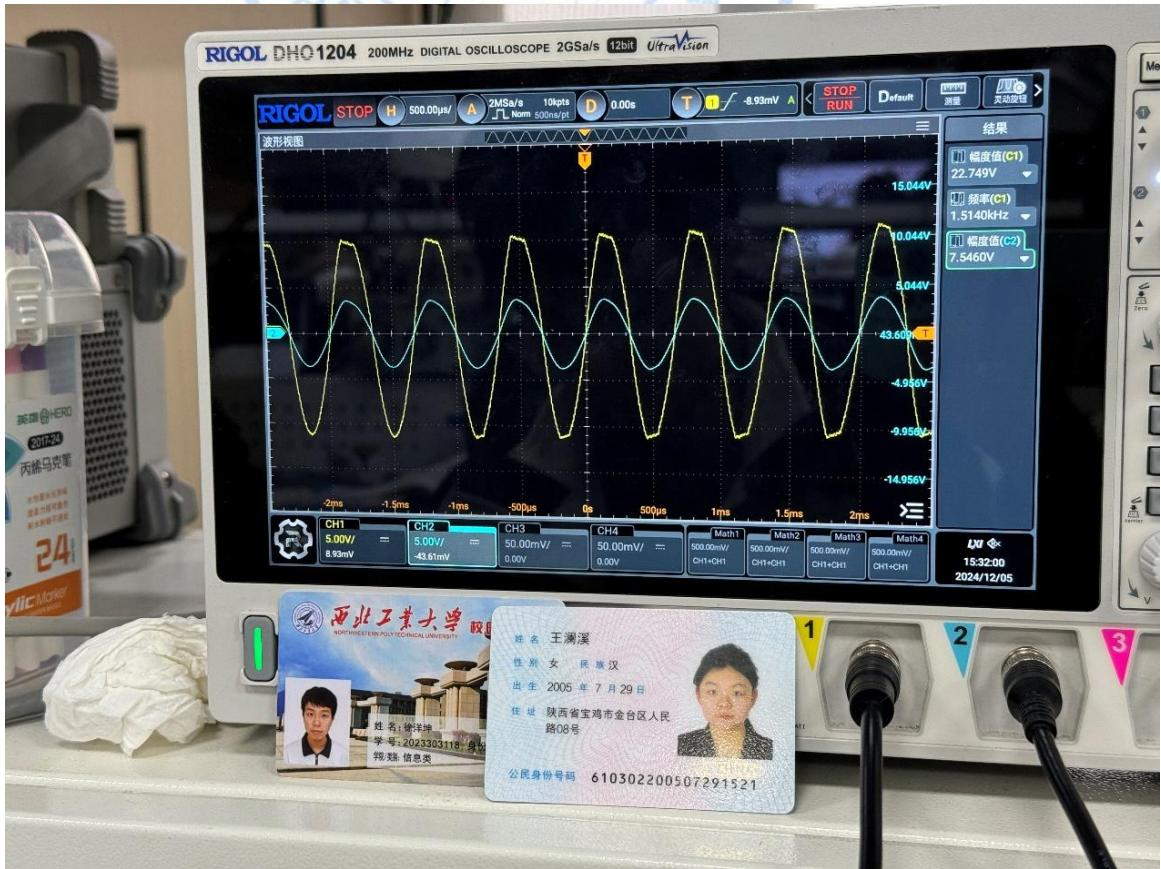
\includegraphics[keepaspectratio]{images/b8640a71ec04a8d08fff8b92b4eacc74235366badac99b2d55355644615dcaa3.jpg}}

（2）三种情况下的测试数据

\begin{longtable}[]{@{}|l|l|l|l|@{}}
\toprule\noalign{}
\endhead
\bottomrule\noalign{}
\endlastfoot
\hline
& 起振 & 振幅最大且不失真 & 临界失真 \\
\hline
可变电阻Rp/kΩ & 4.749 & 8.792 & 9.203 \\
\hline
反馈电压 vfp/V & 0.616 & 6.639 & 7.546 \\
\hline
输出电压 vop/V & 1.777 & 19.968 & 22.749 \\
\hline
\end{longtable}

表1.1

（3）当 \(\mathrm{Rp} = 8.643\mathrm{k}\Omega\)
时两种电容值情况下输出波形

\begin{enumerate}
\def\labelenumi{\Alph{enumi}.}
\tightlist
\item
  \(C_{1} = C_{2} = 0.01 \mu \mathrm{F}\)
\end{enumerate}

\pandocbounded{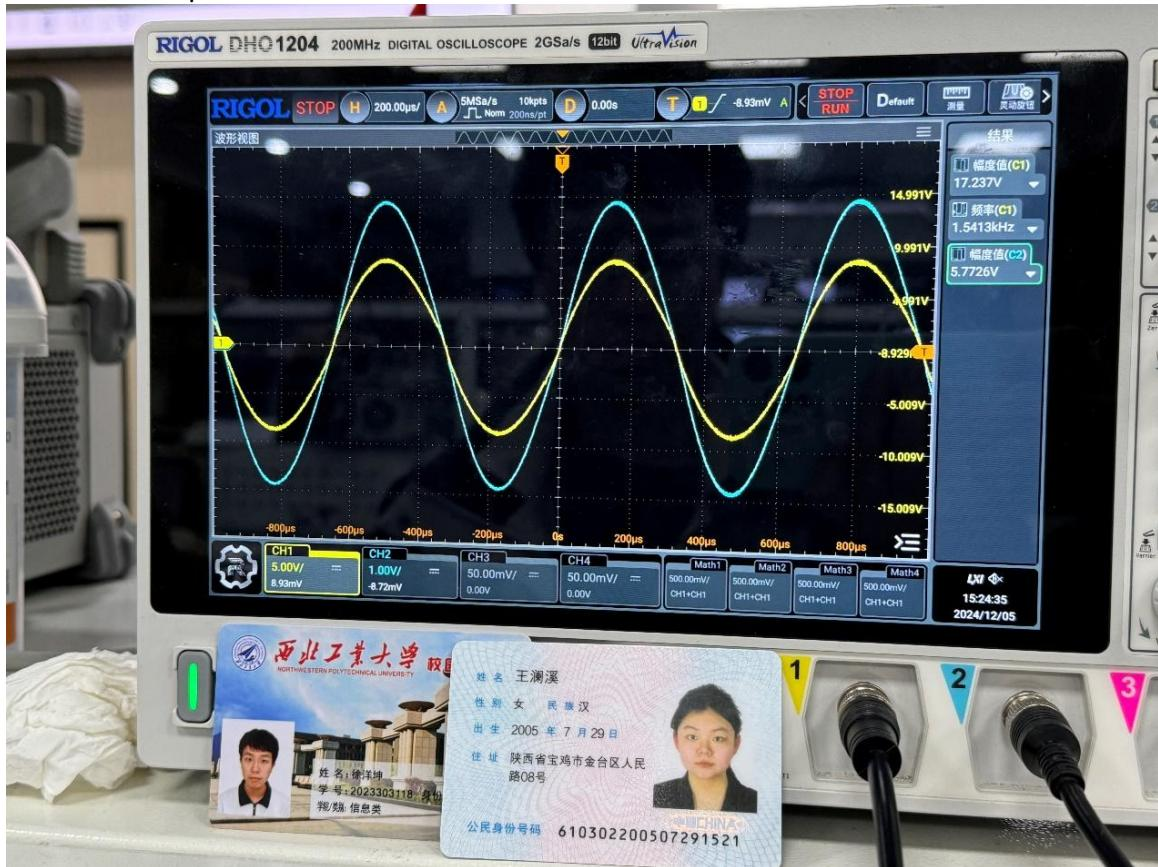
\includegraphics[keepaspectratio]{images/4bb910f29a870938576521ff0fb31090d7f28bae21c4c9937761b9b66379c7a7.jpg}}

\begin{enumerate}
\def\labelenumi{\Alph{enumi}.}
\setcounter{enumi}{1}
\tightlist
\item
  \(C_{1} = C_{2} = 0.02 \mu \mathrm{F}\)
\end{enumerate}

\pandocbounded{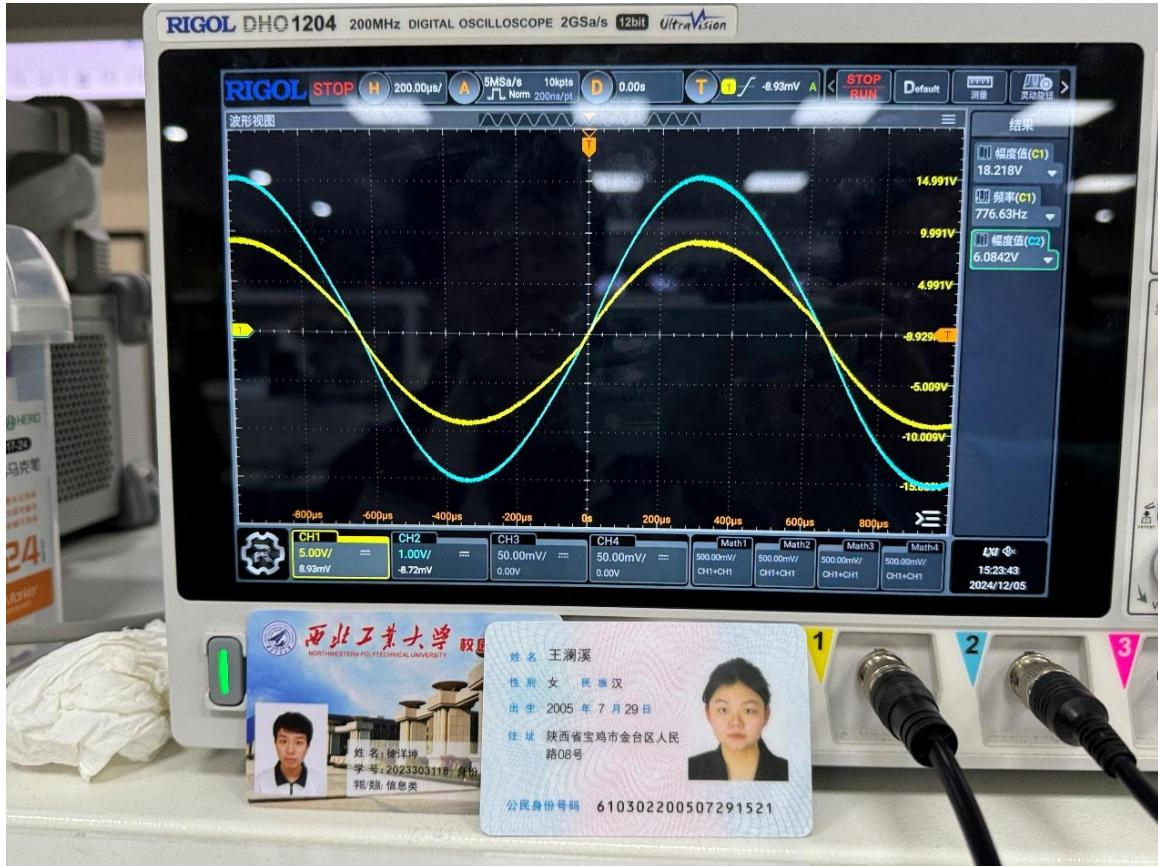
\includegraphics[keepaspectratio]{images/ad7da5abe3698d7f4d05396b7d12f5c9aaf790cf9dbe46f9b9f1b023c8a66c16.jpg}}

（4）当 \(\mathrm{Rp} = 8.643\mathrm{k}\Omega\)
时两种电容值情况下输出波测试数据

\begin{longtable}[]{@{}|l|l|l|l|l|l|l|@{}}
\toprule\noalign{}
\endhead
\bottomrule\noalign{}
\endlastfoot
\hline
& \multicolumn{3}{l}{%
理论值} & \multicolumn{3}{l@{}}{%
实测值} \\
\hline
& 输出电压 vop/V & 频率 f/Hz & 反馈电压 Vf/V & 输出电压 vop/V & 频率
f/Hz & 反馈电压 Vf/V \\
\hline
C1=C2=0.01μF & 17.432 & 1.5915k & 5.634 & 17.237 & 1.5413k & 5.773 \\
\hline
C1=C2=0.02μF & 18.125 & 795.77 & 6.183 & 18.218 & 776.63 & 6.0842 \\
\hline
\end{longtable}

表 1.2

\section{六、结论与分析}\label{ux516dux7ed3ux8bbaux4e0eux5206ux6790-3}

1.数据分析：由表1.1可知当可变电阻值为 \(8.792\mathrm{k}\Omega\)
时输出波形振幅最大且不失真，此时反馈电压 \(\mathbf{V}_{\mathrm{fp}}\)
值为6.639V，输出电压 \(\mathbf{v}_{\mathrm{op}}\)
值为19.968V；由表1.2可知当 \(\mathrm{Rp} = 8.643\mathrm{k}\Omega\)
时输出电压、频率、反馈电压的理论值和实测值误差较小，故可基本认为实验值与计算值相等。\\
2.
实验分析：由上述实验的得出的结果可知，实验误差较小，故可基本认为实验值与计算值相等。\\
3.
实际误差讨论：手动调试示波器到临界失真条件时，不能很好的掌握波形输出恰好在临界点导致测量的输出电压与理论值有误差，在操作时应尽量多调试几次找到波形最合适的点

\section{实验六、有源滤波器}\label{ux5b9eux9a8cux516dux6709ux6e90ux6ee4ux6ce2ux5668}

\section{一、实验目的}\label{ux4e00ux5b9eux9a8cux76eeux7684-4}

1.学习有源滤波器中低通滤波器和带阻滤波器的构成和搭建\\
2. 认识它们的工作原理和优缺点，学会正确在电路中运用\\
3. 观察它们的截止频率，更好的认识二者的频率特性

\section{二、实验原理}\label{ux4e8cux5b9eux9a8cux539fux7406-4}

\section{1.低通滤波器(LPF)：}\label{ux4f4eux901aux6ee4ux6ce2ux5668lpf}

用来通过低频信号,衰减或抑制高频信号的滤波器称为低通滤波器;如图1.1所示为典型的二阶有源低通滤波器。它由两级RC滤波环节与同相比例运算电路组成,其中第一级电容C1接至输出端,通过引人适量的正反馈,以改善幅频特性。描述电路性能的参数有:

二阶低通滤波器的通带增益为：

\[
A v f = 1 + \frac {R f}{R 3}
\]

为保证电路不出现自激, 应限制电路的增益不能太高.

若
\(\mathrm{R1} = \mathrm{R2} = \mathrm{R},\mathrm{C1} = \mathrm{C2} = \mathrm{C}\)
，则上限截止频率为：

\[
f H = f 0 = \frac {1}{2 \pi R C}
\]

品质因数Q是衡量滤波器选择性的一个指标。其大小影响低通滤波器在截止频率处幅频特性的形状。Q值越大,则随频率变化,增益衰减越快。

\[
Q = \frac {1}{3 - A v f}
\]

\section{2. 带阻滤波器(BEF):}\label{ux5e26ux963bux6ee4ux6ce2ux5668bef}

在双T网络后加一级同相比例运算电路就构成了基本的二阶有源带阻滤波器,如图1.2所示。这种电路的性能和带通滤波器相反,即在规定的频带内,信号不能通过(或受到很大衰减或抑制),而在其余频率范围,信号则能顺利通过。描述电路性能的参数有:

通带增益为

\[
A v f = 1 + \frac {R f}{R 3}
\]

若 \(\mathrm{R1 = R2 = 2R4 = R}\) ，0.5C1
\(= \mathrm{C2} = \mathrm{C3} = \mathrm{C}\) ，则截止频率为

\[
f 0 = \frac {1}{2 \pi R C}
\]

带阻滤波器的通带截止频率有两个，分别为

\[
f L = f 0 [ \sqrt {(2 - A v f) ^ {2} + 1} - (2 - A v f) ]
\]

\[
f H = f 0 [ \sqrt {(2 - A v f) ^ {2} + 1} + (2 - A v f) ]
\]

带阻带宽

\[
f _ {B W} = f 2 - f 1 = 2 f 0 \left(2 - A _ {V f}\right)
\]

品质因数为

\[
Q = \frac {1}{2 (2 - A _ {V f})}
\]

带阻滤波器在检测仪表中应用较多，常用于滤除 \(50\mathrm{Hz}\)
交流电源引起的干扰信号。这时带阻的中心频率选为 \(50\mathrm{Hz}\)
，使对应于该中心频率的电压放大倍数为零。

\section{三、实验内容}\label{ux4e09ux5b9eux9a8cux5185ux5bb9-4}

\section{1.低通滤波器}\label{ux4f4eux901aux6ee4ux6ce2ux5668}

（1）取 \(\mathbf{v}\)
为峰值为1V的正弦波信号，调整输入信号的频率，分别测量输入频率在
\(100\mathrm{Hz},150\mathrm{Hz},200\mathrm{Hz},\dots ,1000\mathrm{Hz}\)
时输出电压的大小，记入表1.1中。\\
（2）根据所记录的数据，计算电压放大倍数，记入表1.1中。\\
（3）根据所计算的增益，作出频率特性图(Av-f图)，并估算滤波器的上限频率f。

（4）固定输入信号电压的幅值不变，调节其频率，直到输出波形的峰峰值为通带时峰峰值的0.707时，记录下此时函数信号发生器输出信号的频率f。

\section{2.带阻滤波器}\label{ux5e26ux963bux6ee4ux6ce2ux5668}

（1）取u为峰值为1V的正弦波信号，调整输入信号的频率，分别测量输入频率在
\(100\mathrm{Hz},150\mathrm{Hz},200\mathrm{Hz},\dots ,1000\mathrm{Hz}\)
时输出电压的大小，记人表1.2中。\\
（2）根据所记录的数据，计算电压放大倍数，记入表1.2中。\\
（3）根据所计算的增益，作出频率特性图(Av-f图)，并估算滤波器的下限频率fL和上限频率fH。\\
（4）固定输入信号电压的幅值不变，调节其频率，直到输出波形的峰峰值为通带时峰峰值的0.707时，记录下此时示波器所示的信号频率f和fH。

\section{四、实验电路方案}\label{ux56dbux5b9eux9a8cux7535ux8defux65b9ux6848-4}

\section{1. 低通滤波器}\label{ux4f4eux901aux6ee4ux6ce2ux5668-1}

\pandocbounded{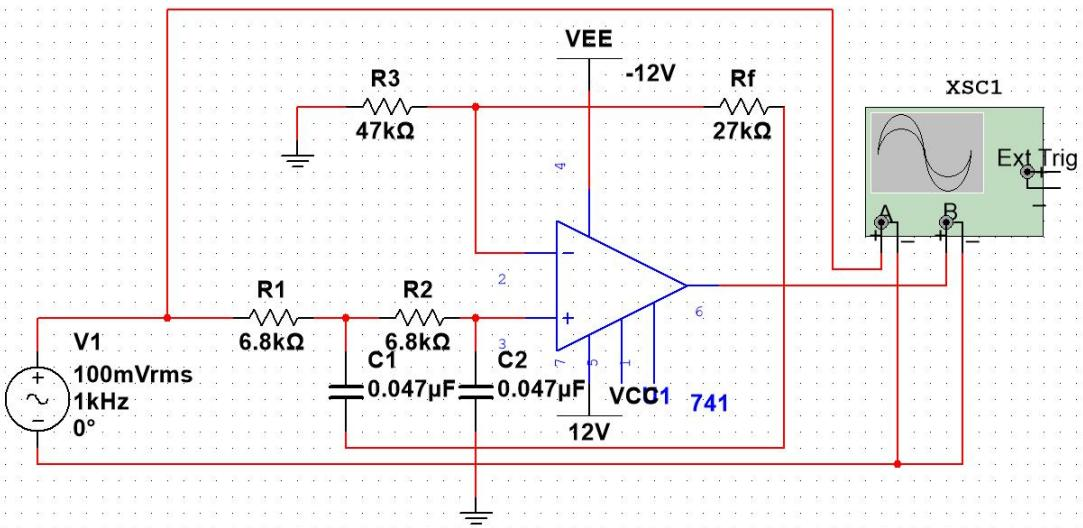
\includegraphics[keepaspectratio]{images/97e12689d57edb1a026cc4225a1b211df42af507e4fc0a5aea1e2442c830bb36.jpg}}\\
图1.1

\section{2. 带阻滤波器}\label{ux5e26ux963bux6ee4ux6ce2ux5668-1}

\pandocbounded{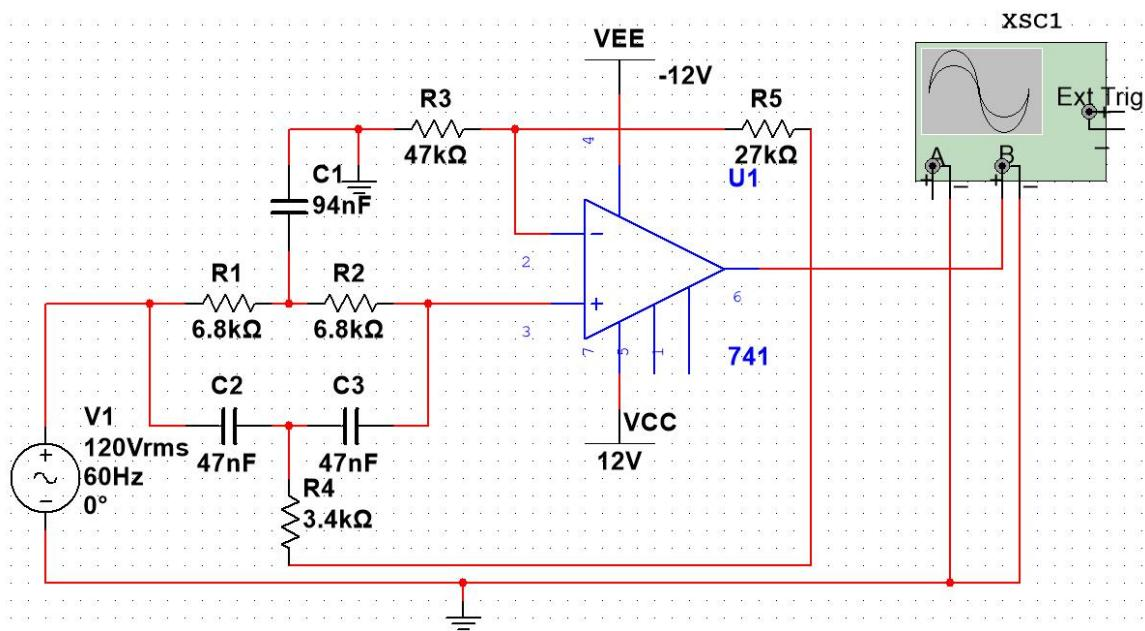
\includegraphics[keepaspectratio]{images/727872af55a44e3c93cfe571153e482ba267a544b423385beb4031202890537c.jpg}}

\section{五、测试与数据记录}\label{ux4e94ux6d4bux8bd5ux4e0eux6570ux636eux8bb0ux5f55-4}

\section{1. 测试用仪器}\label{ux6d4bux8bd5ux7528ux4eeaux5668-4}

面包板，示波器，741放大器，导线、电阻、电感、电容若干。

\section{2. 数据记录}\label{ux6570ux636eux8bb0ux5f55-2}

\section{\texorpdfstring{（1）低通滤波器
\((\mathrm{vi} = 1\mathrm{V})\)}{（1）低通滤波器 (\textbackslash mathrm\{vi\} = 1\textbackslash mathrm\{V\})}}\label{ux4f4eux901aux6ee4ux6ce2ux5668-mathrmvi-1mathrmv}

A.表格数据记录

\begin{longtable}[]{@{}|l|l|l|l|l|l|l|l|l|l|@{}}
\toprule\noalign{}
\endhead
\bottomrule\noalign{}
\endlastfoot
\hline
输入频率 /Hz & 100 & 150 & 200 & 250 & 300 & 400 & 600 & 800 & 1000 \\
\hline
Vop/V & 1.62 & 1.67 & 1.62 & 1.66 & 1.55 & 1.45 & 1.07 & 0.86 & 0.77 \\
\hline
Av/(vo/vi) & 1.62 & 1.67 & 1.62 & 1.66 & 1.55 & 1.45 & 1.07 & 0.86 &
0.77 \\
\hline
Av/dB & 2.10 & 2.23 & 2.10 & 2.20 & 1.90 & 1.61 & 0.29 & -0.66 &
-1.14 \\
\hline
\end{longtable}

B.频率特性图（Av-f图）

\pandocbounded{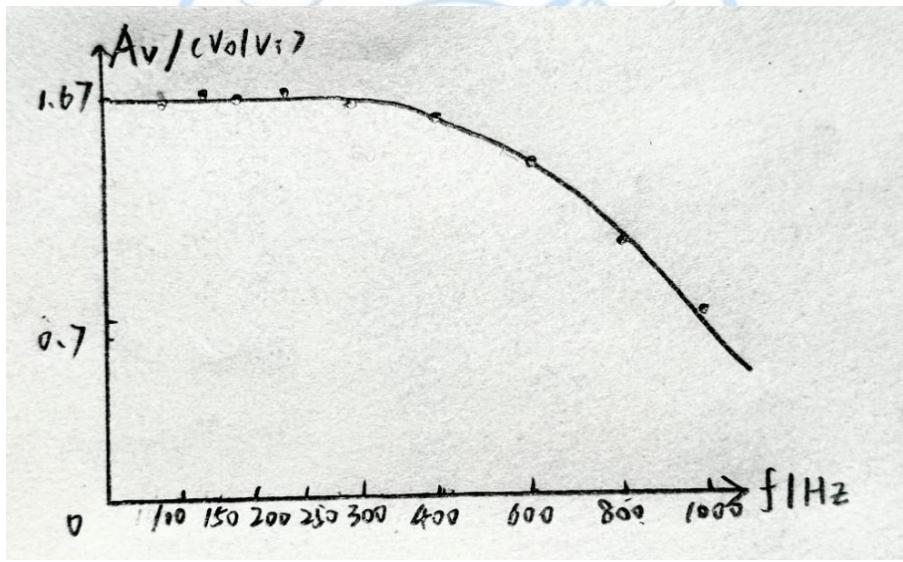
\includegraphics[keepaspectratio]{images/81e399bd26953a9f649c466cbab9b3691e69f75479b500636c1cad56ee5ee1a0.jpg}}\\
图1.2\\
表1.1\\
图1.3

C. 输出波形的峰峰值为通带时峰峰值的 0.707 时,
\(\mathrm{{fH}} = {530}\mathrm{\;{Hz}}\) ; 由

\[
f H = f 0 = \frac {1}{2 \pi R C}
\]

计算得fH理论值为 \(498\mathrm{Hz}\)

\section{\texorpdfstring{（2）带阻滤波器
\((\mathrm{vi} = 1\mathrm{V})\)}{（2）带阻滤波器 (\textbackslash mathrm\{vi\} = 1\textbackslash mathrm\{V\})}}\label{ux5e26ux963bux6ee4ux6ce2ux5668-mathrmvi-1mathrmv}

A.表格数据记录

\begin{longtable}[]{@{}|l|l|l|l|l|l|l|l|l|l|@{}}
\toprule\noalign{}
\endhead
\bottomrule\noalign{}
\endlastfoot
\hline
输入频率 /Hz & 100 & 150 & 200 & 250 & 300 & 400 & 600 & 800 & 1000 \\
\hline
Vop/V & 1.56 & 1.52 & 1.46 & 1.36 & 1.23 & 0.79 & 0.51 & 1.13 & 1.35 \\
\hline
Av/(vo/vi) & 1.56 & 1.52 & 1.46 & 1.36 & 1.23 & 0.79 & 0.51 & 1.13 &
1.35 \\
\hline
Av/dB & 1.93 & 1.82 & 1.64 & 1.34 & 0.90 & -1.02 & -2.92 & 0.53 &
1.30 \\
\hline
\end{longtable}

表1.2

B.频率特性图（Av-f图）

\pandocbounded{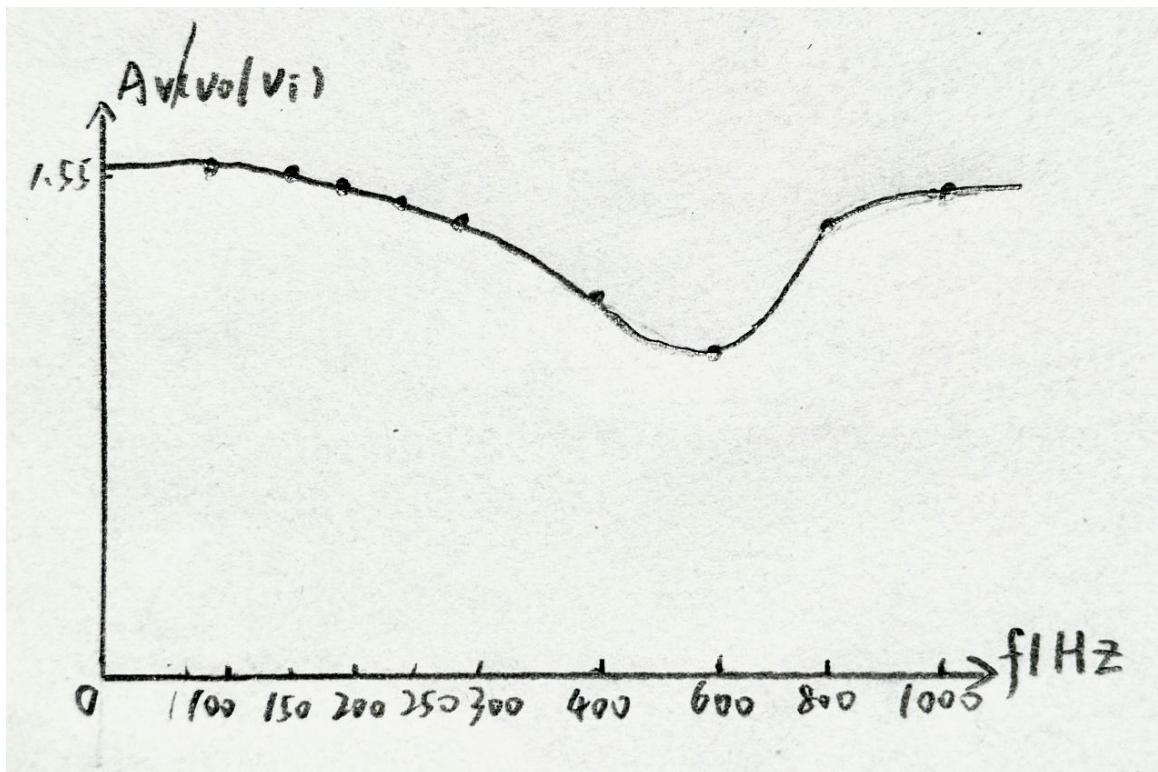
\includegraphics[keepaspectratio]{images/07d83ecc01e1086e3f78a4fd8a4e4ae2bb8d42efe78e2216ab0c8934abbd81f5.jpg}}\\
图1.4

C. 输出波形的峰峰值为通带时峰峰值的 0.707 时,
\(\mathrm{fL} = {332}\mathrm{{Hz}},\mathrm{{fH}} = {792}\mathrm{{Hz}}\)
; 由

\[
f H = f 0 = \frac {1}{2 \pi R C}
\]

计算得fL理论值为 \(328\mathrm{Hz}\) ，fH理论值为 \(756\mathrm{Hz}\)

\section{六、结论与分析}\label{ux516dux7ed3ux8bbaux4e0eux5206ux6790-4}

\begin{enumerate}
\def\labelenumi{\arabic{enumi}.}
\tightlist
\item
  数据分析：由表 1.1 可知当低通滤波器输出波形的峰峰值为通带时峰峰值的
  0.707 时， \(f_{\mathrm{H}} = 530 \mathrm{~Hz}\) ；，而理论值
  \(f = 498 \mathrm{~Hz}\) ；由表 1.2
  可知当带阻滤波器输出波形的峰峰值为通带时峰峰值的 0.707 时，
  \(f_{\mathrm{L}} = 332 \mathrm{~Hz}\) ，
  \(f_{\mathrm{H}} = 792 \mathrm{~Hz}\) ；，而理论值
  \(f_{\mathrm{L}} = 328 \mathrm{~Hz}\) ，
  \(f_{\mathrm{H}} = 756 \mathrm{~Hz}\)
  ；理论值和实测值误差不大，故可基本认为实验值与计算值相等。\\
\item
  实验分析：由上述实验的得出的结果可知，实验误差较小，故可基本认为实验值与计算值相等。\\
\item
  实际误差讨论：频率取样间隔较大，导致得到的截止频率可能不完全准确；原件不齐全，拿其他参数原件代替接入电路产生误差
\end{enumerate}

\section{实验七、全波整流滤波}\label{ux5b9eux9a8cux4e03ux5168ux6ce2ux6574ux6d41ux6ee4ux6ce2}

\section{一、实验目的}\label{ux4e00ux5b9eux9a8cux76eeux7684-5}

(1)掌握单相全波整流电路的工作原理与测试方法。\\
(2)学会正确使用示波器和万用表,测量并分析输人输出电压波形及数量关系\\
(3)学会几种不同整流电路的波形测量。\\
(4)分析各种滤波电路的特点及对整流波形的影响。

\section{二、实验原理}\label{ux4e8cux5b9eux9a8cux539fux7406-5}

\section{单相全波整流滤波电路}\label{ux5355ux76f8ux5168ux6ce2ux6574ux6d41ux6ee4ux6ce2ux7535ux8def}

与半波整流不同的是，变压器多了一个中间抽头，其 \(1\sim 0\) 绕组与
\(0\sim 2\) 绕组匝数相等。

由于变压器次级有中间抽头,因此,变压器次级感应电压被分为两部分:v2a和v2b。v2a由变压器次级1\textsubscript{0绕组产生；v2b由变压器次级0}2绕组产生。当输入交流电压vi为正半周时，二极管D1因正偏而导通(相当于开关接通)，电流自上而下流经负载RL到变压器器中心抽头0端;二极管D2因反偏而截止(相当于开关断开)。当输入交流电压vi为负半周时,D1截止、D2导通，电流仍自上而下流经负载RL到变压器器中心抽头0端。

当交流电进人下一个周期时，又重复上述过程。可见，交流电的正负半周使D1与D2轮流导通，在负载上总是得到自上而下的单向脉动直流电流。与半波整流相比，它有效地利用了交流电的负半周。全波整流波形如图1.1所示，全波整流电路的输出电压
\(\mathrm{Vo} = 0.9\mathrm{v}2\) ：比半波整流提高了一倍。

当在负载两端并接上电容C滤波时，其输出电压更加平稳。

\section{三、实验内容}\label{ux4e09ux5b9eux9a8cux5185ux5bb9-5}

使用信号源产生全波整流的输入信号VI，其为正弦波，频率为 \(1\mathrm{kHz}\)
，2V峰峰值，偏移电压0V。使用普通二极管整流电路进行全波整流，用示波器两个通道分别测试
\(\mathrm{Vo}+\) 对地波形以及 \(\mathrm{Vo}-\)
对地波形，并用示波器的math功能，用 \(\mathrm{Vo}+\) 减去
\(\mathrm{Vo}-\)
，得到差值即为二极管整流电路的输出波形，并测量输出波形及参数。

\section{四、实验电路方案}\label{ux56dbux5b9eux9a8cux7535ux8defux65b9ux6848-5}

\pandocbounded{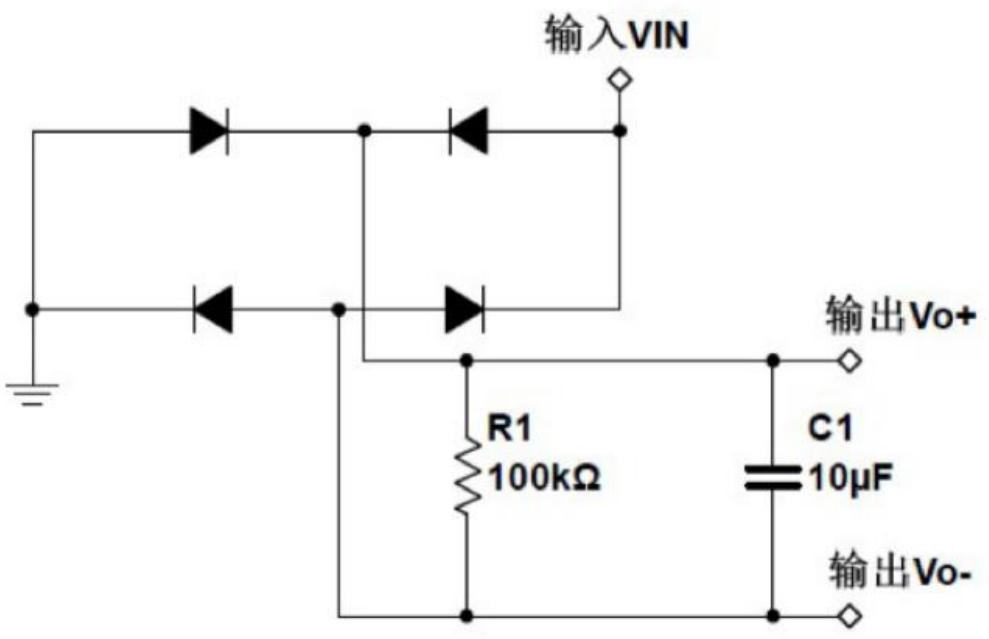
\includegraphics[keepaspectratio]{images/cbb170de72b6959c3abca2d2984015c8838e3291d93df170c15414c1df1f2917.jpg}}\\
图1.1

\section{五、测试与数据记录}\label{ux4e94ux6d4bux8bd5ux4e0eux6570ux636eux8bb0ux5f55-5}

\begin{enumerate}
\def\labelenumi{\arabic{enumi}.}
\tightlist
\item
  二极管整流电路的输出波形
\end{enumerate}

A. 两输出原始波形

\pandocbounded{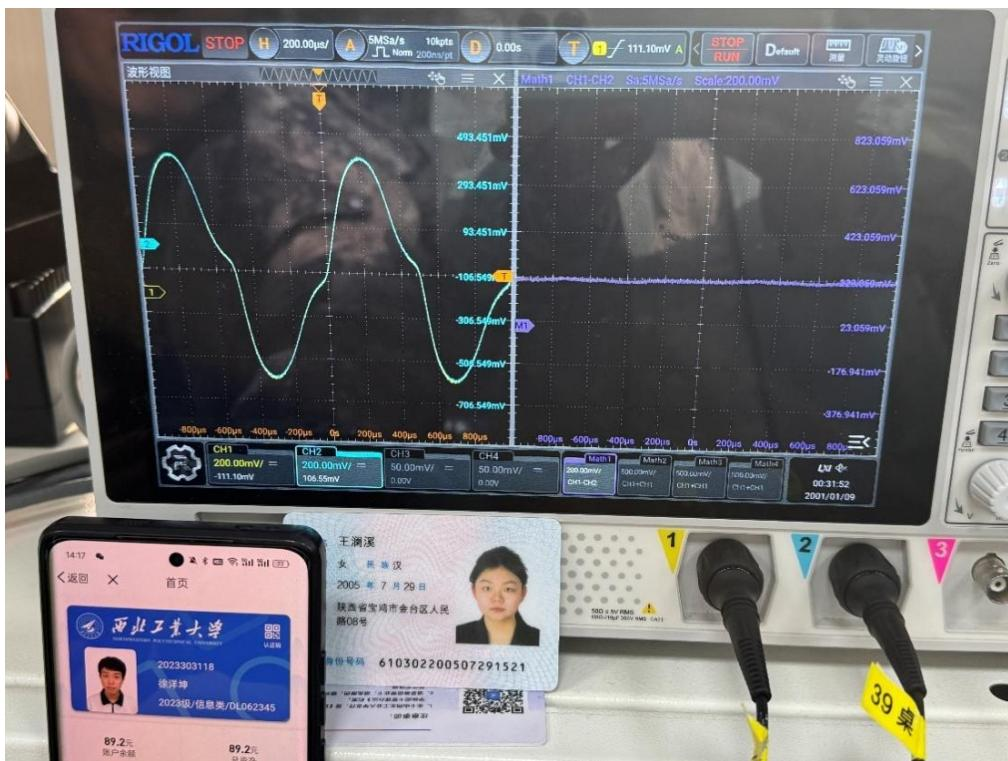
\includegraphics[keepaspectratio]{images/72cc6fdf266719508a361a75418a78ce5056e4f59762856fd7c8f82c66384398.jpg}}\\
图1.2

\pandocbounded{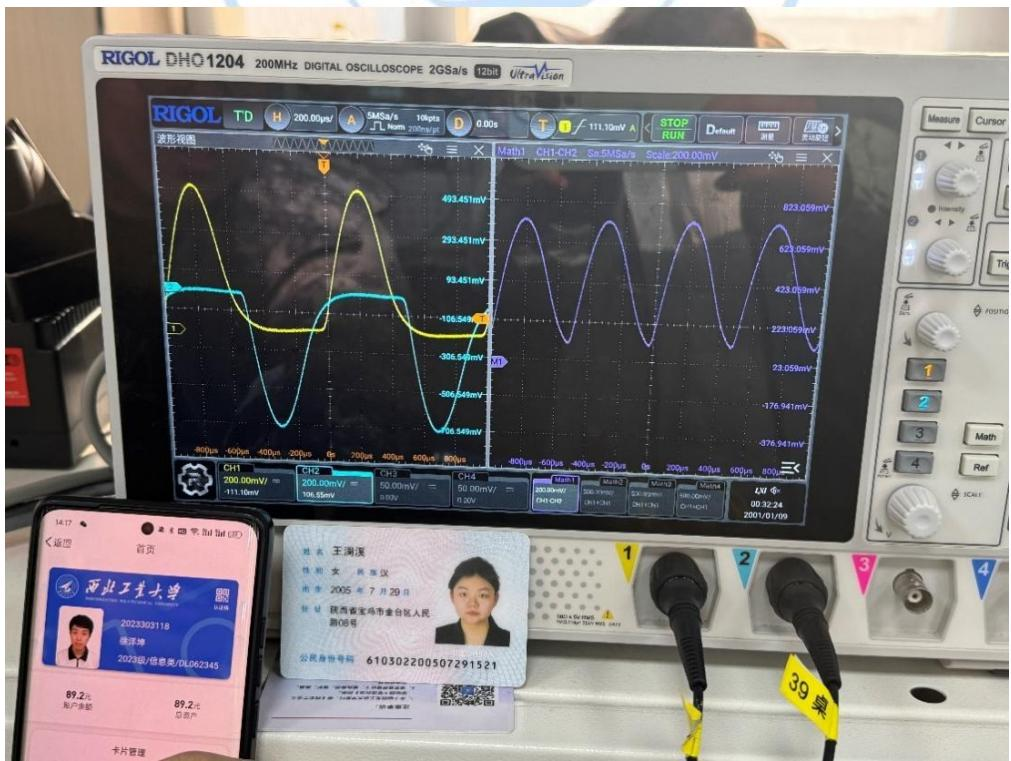
\includegraphics[keepaspectratio]{images/16d343362737aebecdc166d2dcd93068074d1b475d50c8593d29c95b6570b755.jpg}}\\
B. 用示波器math相减处理后\\
图1.3

\section{六、结论与分析}\label{ux516dux7ed3ux8bbaux4e0eux5206ux6790-5}

根据图1.3可得单相全波整流电路能实现交流电在整个周期内的输出，负载上总能得到带向脉动直流电流，与半波整流相比有效地利用了交流电的负半周，输出电压
\(\mathrm{Vo} = 0.9\mathrm{V}2\) 比半波整流提高了一倍

\section{实验八、功率放大电路}\label{ux5b9eux9a8cux516bux529fux7387ux653eux5927ux7535ux8def}

\section{一、实验目的}\label{ux4e00ux5b9eux9a8cux76eeux7684-6}

\begin{enumerate}
\def\labelenumi{\arabic{enumi}.}
\tightlist
\item
  了解功率放大器的工作原理及主要性能指标的意义；\\
  2.学会集成功率放大器的使用及主要性能指标的测试；
\end{enumerate}

\section{二、实验原理}\label{ux4e8cux5b9eux9a8cux539fux7406-6}

\section{1.
功率放大器类型}\label{ux529fux7387ux653eux5927ux5668ux7c7bux578b}

\section{（1）A类}\label{aux7c7b}

输出功率管始终处于导通状态，无输入信号时，输出级导通存在直流电流。优点：失真小，波形平滑；缺点：功耗大，效率低，发热大

\section{（2）B类}\label{bux7c7b}

当无输入时，输出晶体管不导通，当有输入时，每个输出管各放大一半波形，彼此一开一关轮流工作完成一个全波放大；优点：功耗小，效率较高；缺点：有交越失真

\section{（3）AB类}\label{abux7c7b}

输出级晶体管工作在不同的静态工作点上，在无输入时也有少量电流通过输出晶体管。优点：克服交越失真，失真小；缺点：效率高于A类，低于B类。

\section{（4）D类}\label{dux7c7b}

D 类:输入信号经过脉冲宽度调制, 产生脉冲宽度波形控制输出级开关管输出功率,
经过 LC 滤波器得到最终输出信号。

\section{2.互补对称功率放大电路}\label{ux4e92ux8865ux5bf9ux79f0ux529fux7387ux653eux5927ux7535ux8def}

(1)双电源互补对称功率放大电路(Output Capacitor
Less,OCL,无输出电容电路)。采用正、负两个直流电源供电的互补对称电路称为双电源电路。一般这两个直流电源大小相同，极性相反。

乙类双电源互补对称功率放大电路：低频功放采用乙类工作状态可以提高效率。但功放管处于乙类工作状态时，管子静态工作电流为零，输出波形将被削去一半，这将产生严重的非线性失真。为解决效率和失真的矛盾，可以选用两只互补的三极管(NPN管Q和PNP管Q2，特性完全相同的异型晶体管)，使它们都工作在乙类状态。两只晶体管轮流工作，一只晶体管在输入信号正半周导通，另一只晶体管在输入信号负半周导通，最终在负载上合成了一个完整的正弦波周期，从而解决了乙类放大电路存在的效率与失真之间的矛盾。在理想情况下，该电路的正负电源和电路结构完全对称，所以静态时输出端的电压为零不必采用耦合电容来隔直，该电路又叫OCL电路。由于输出端没有耦合电容,OCL电路具有较好的频率特性。

在实际中，乙类双电源互补对称电路并不能使输出电压很好地反映输入电压的变化，因为晶体管输人特性门限电压(NPN
硅管约为 0.6V, PNP 锗管约为 0.2V)
不为零，且电压和电流关系也不是线性关系。在输入电压较低时，输入基极电流很小，故输出电流十分小，负载电阻
R，上无电流通过。因此输出电压在输入电压较小时，存在一小段死区，此段输出电压与输入电压不存在线性关系，产生了失真。由于这种失真出现在通过零值处，因而称为交越失真。

2)甲乙类双电源互补对称功率放大电路。为了克服交越失真,必须在两只功率放大管的基极之间加偏置电压,使功率放大管在静态时均处于临界导通或微导通状态。施加正弦电压信号后,不需克服门限电压而即刻导通。由于两管的导通时间都比输入信号的半个周期长,即在信号电压很小时,两管同时导通,因而它们工作在甲乙类状态,电路称为甲乙类互补对称功率放大电路。

\section{三、实验内容}\label{ux4e09ux5b9eux9a8cux5185ux5bb9-6}

搭建图中所示AB类功放电路，电源使用正负5V供电。二极管使用1N4148，02使用npn，

型号 S8050，03 使用 pnp，型号 S8550。其中 R1 是 AB
类功放电路输出负载，取 20。由于功放输出电流较大，建议在面包板 AB
类输出级的正负电源之间加 10uF 或更大的滤波电容 (注意极性)。

\section{四、实验电路方案}\label{ux56dbux5b9eux9a8cux7535ux8defux65b9ux6848-6}

\pandocbounded{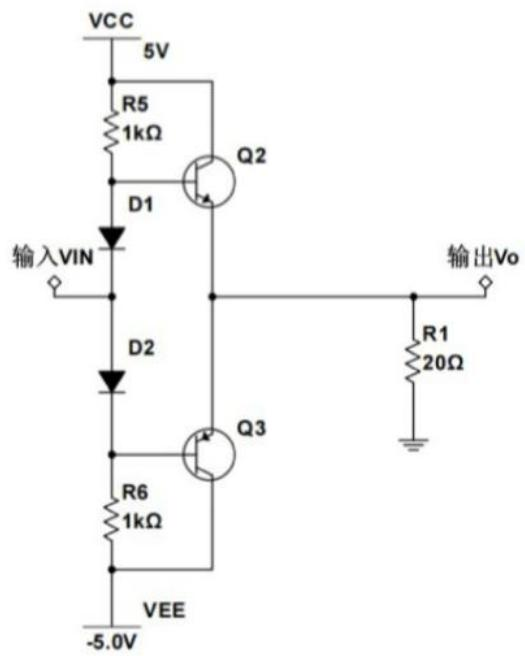
\includegraphics[keepaspectratio]{images/dee819a95d288ac7fa1de3c16f61ec323c488ed92e8aa1005d6f56fb52633913.jpg}}

\section{五、测试与数据记录}\label{ux4e94ux6d4bux8bd5ux4e0eux6570ux636eux8bb0ux5f55-6}

\section{1. 测试用仪器}\label{ux6d4bux8bd5ux7528ux4eeaux5668-5}

直流稳压电源、函数信号发生器、示波器、万用表、集成功放、电阻、电容二极管若干

\section{2. 实验步骤}\label{ux5b9eux9a8cux6b65ux9aa4-4}

(1)输入信号VIN为 \(10\mathrm{kHz}\)
正弦波，峰峰值1V,偏移0V,测试输出电压Vo参数，并根据负载电阻R1值，计算输出功率。\\
(2)拿8Q的喇叭替换AB类功放电路的 \(20\Omega\)
负载电阻，输入信号为VIN为正弦波，偏移0V，分别调整正弦波频率1kHz到10kHz之间，幅度1V到2V之间，听喇叭声音大小和音调，观察其与正弦波参数的关系。(要求(2)内容不用体现在实验报告中)

\section{3. 数据记录}\label{ux6570ux636eux8bb0ux5f55-3}

（1）功放电路输出波形

\pandocbounded{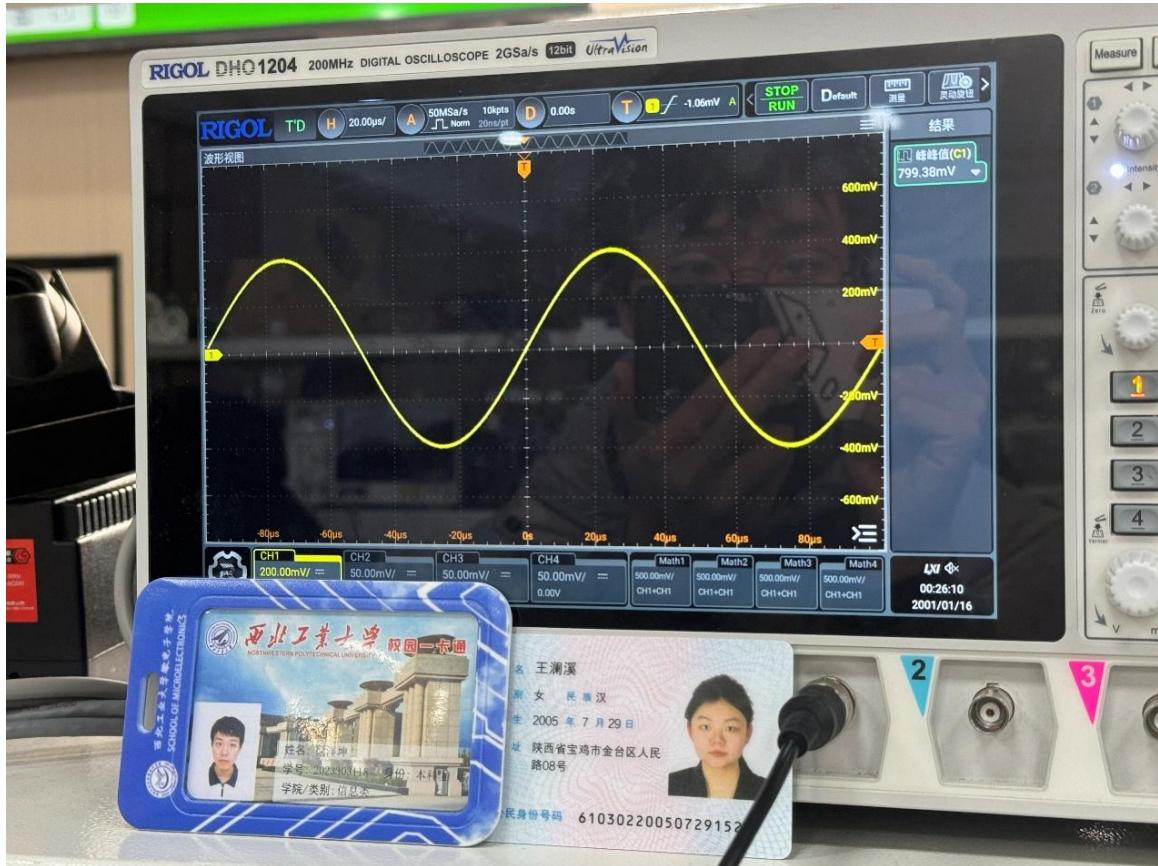
\includegraphics[keepaspectratio]{images/becdfacd4eb840e42c62d6b47460322e6514d44916bdc9d03641ee5a31e09e83.jpg}}\\
图1.2

\pandocbounded{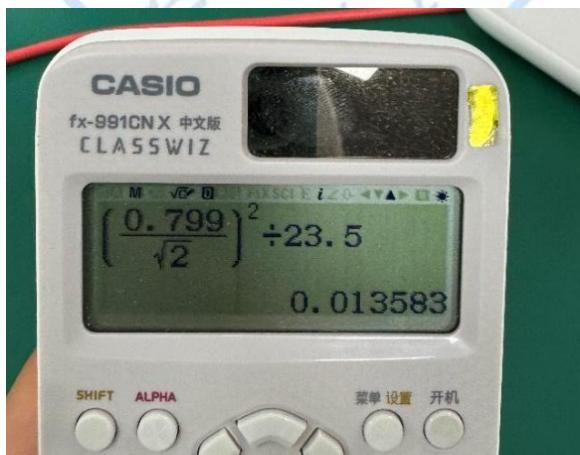
\includegraphics[keepaspectratio]{images/72a9ba1f19bf82cb20e00793ca239c66523cb09da24111974032a41c6a74b24a.jpg}}\\
（2）输出功率计算\\
图1.3

\section{六、结论与分析}\label{ux516dux7ed3ux8bbaux4e0eux5206ux6790-6}

测试出 Vo 值如图 1.2 所示，根据负载电阻 R1
值，结合输出功率计算公式可计算如图 1.3 所示，得到输出功率
\(\mathrm{Po} = 0.014\mathrm{W}\)

\end{document}
